%%% The main file. It contains definitions of basic parameters and includes all other parts.

%% Settings for single-side (simplex) printing
% Margins: left 40mm, right 25mm, top and bottom 25mm
% (but beware, LaTeX adds 1in implicitly)
%\documentclass[12pt,a4paper]{report}
%\setlength\textwidth{145mm}
%\setlength\textheight{247mm}
%\setlength\oddsidemargin{15mm}
%\setlength\evensidemargin{15mm}
%\setlength\topmargin{0mm}
%\setlength\headsep{0mm}
%\setlength\headheight{0mm}
% \openright makes the following text appear on a right-hand page
%\let\openright=\clearpage

%% Settings for two-sided (duplex) printing
\documentclass[12pt,a4paper,twoside,openright]{report}
% \setlength\textwidth{145mm}
% \setlength\textheight{247mm}
% \setlength\oddsidemargin{14.2mm}
% \setlength\evensidemargin{0mm}
% \setlength\topmargin{0mm}
% \setlength\headsep{0mm}
% \setlength\headheight{0mm}
\let\openright=\cleardoublepage

%% Character encoding: usually latin2, cp1250 or utf8:
\usepackage[utf8]{inputenc}


%% Further useful packages (included in most LaTeX distributions)
\usepackage{amsmath}        % extensions for typesetting of math
\usepackage{amsfonts}       % math fonts
\usepackage{amsthm}         % theorems, definitions, etc.
%\usepackage{bbding}         % various symbols (squares, asterisks, scissors, ...)
%\usepackage{bm}             % boldface symbols (\bm)
\usepackage{graphicx}       % embedding of pictures
\usepackage{caption}       % embedding of pictures
\usepackage{subcaption}       % embedding of pictures
%\usepackage{fancyvrb}       % improved verbatim environment
%\usepackage[square]{natbib}         % citation style AUTHOR (YEAR), or AUTHOR [NUMBER]
%\usepackage[nottoc]{tocbibind} % makes sure that bibliography and the lists
			    % of figures/tables are included in the table
			    % of contents
%\usepackage{dcolumn}        % improved alignment of table columns
%\usepackage{booktabs}       % improved horizontal lines in tables
%\usepackage{paralist}       % improved enumerate and itemize
\usepackage{tikz}
\usetikzlibrary{shapes,fit,positioning,snakes,mindmap,trees,decorations.text,arrows.meta}
\usepackage{gnuplot-lua-tikz}
\usepackage{nomencl}
\usepackage{epigraph}
\makenomenclature
\usepackage{algorithm,algpseudocode}
\usepackage{enumitem}
\usepackage{booktabs}
\usepackage[a-2u]{pdfx}
\setitemize{itemsep=0pt}
%\usepackage[usenames]{xcolor}  % typesetting in color
\usepackage[textsize=tiny]{todonotes}
\newcommand{\XX}[1]{\textcolor{red}{#1}}

%%% Basic information on the thesis

% Thesis title in English (exactly as in the formal assignment)
\def\ThesisTitle{Traffic scheduler for Differentiated Services}

% Author of the thesis
\def\ThesisAuthor{Michal Bali}

% Year when the thesis is submitted
\def\YearSubmitted{2018}

% Name of the department or institute, where the work was officially assigned
% (according to the Organizational Structure of MFF UK in English,
% or a full name of a department outside MFF)
\def\Department{Department of Software Engineering}

% Is it a department (katedra), or an institute (ústav)?
\def\DeptType{Department}

% Thesis supervisor: name, surname and titles
\def\Supervisor{Miroslav Kratochvíl, M.Sc.}

% Supervisor's department (again according to Organizational structure of MFF)
\def\SupervisorsDepartment{Department of Software Engineering}

% Study programme and specialization
\def\StudyProgramme{Computer Science}
\def\StudyBranch{General Computer Science}

\setlength\epigraphwidth{9cm}
\setlength\epigraphrule{0pt}

% An optional dedication: you can thank whomever you wish (your supervisor,
% consultant, a person who lent the software, etc.)
\def\Dedication{%

%\epigraph{}

%\noindent

%\emph{}.

%\vspace{3 ex}
%\noindent
I would also like to thank my supervisor Mirek Kratochvíl.
}

% Abstract (recommended length around 80-200 words; this is not a copy of your thesis assignment!)
\def\Abstract{%
Lorem ipsum
}

% 3 to 5 keywords (recommended), each enclosed in curly braces
\def\Keywords{%
{computer networks} {internet} {network traffic scheduling} {active queue management}
}



%% The hyperref package for clickable links in PDF and also for storing
%% metadata to PDF (including the table of contents).
%\usepackage[pdftex,unicode]{hyperref}   % Must follow all other packages
%\hypersetup{breaklinks=true}
%\hypersetup{pdftitle={\ThesisTitle}}
%\hypersetup{pdfauthor={\ThesisAuthor}}
%\hypersetup{pdfkeywords=\Keywords}
%\hypersetup{urlcolor=blue}

% Definitions of macros (see description inside)
%%% This file contains definitions of various useful macros and environments %%%
%%% Please add more macros here instead of cluttering other files with them. %%%

%%% Minor tweaks of style

% These macros employ a little dirty trick to convince LaTeX to typeset
% chapter headings sanely, without lots of empty space above them.
% Feel free to ignore.
\makeatletter
\def\@makechapterhead#1{
  {\parindent \z@ \raggedright \normalfont
   \Huge\bfseries \thechapter. #1
   \par\nobreak
   \vskip 20\p@
}}
\def\@makeschapterhead#1{
  {\parindent \z@ \raggedright \normalfont
   \Huge\bfseries #1
   \par\nobreak
   \vskip 20\p@
}}
\makeatother

% This macro defines a chapter, which is not numbered, but is included
% in the table of contents.
\def\chapwithtoc#1{
\chapter*{#1}
\addcontentsline{toc}{chapter}{#1}
}

% Draw black "slugs" whenever a line overflows, so that we can spot it easily.
\overfullrule=1mm

%%% Macros for definitions, theorems, claims, examples, ... (requires amsthm package)

\theoremstyle{plain}
\newtheorem{thm}{Theorem}
\newtheorem{lemma}[thm]{Lemma}
\newtheorem{claim}[thm]{Claim}

\theoremstyle{plain}
\newtheorem{defn}{Definition}

\theoremstyle{remark}
\newtheorem*{cor}{Corollary}
\newtheorem*{rem}{Remark}
\newtheorem*{observation}{Observation}
\newtheorem*{example}{Example}

%%% An environment for proofs

%%% FIXME %%% \newenvironment{proof}{
%%% FIXME %%%   \par\medskip\noindent
%%% FIXME %%%   \textit{Proof}.
%%% FIXME %%% }{
%%% FIXME %%% \newline
%%% FIXME %%% \rightline{$\square$}  % or \SquareCastShadowBottomRight from bbding package
%%% FIXME %%% }

%%% An environment for typesetting of program code and input/output
%%% of programs. (Requires the fancyvrb package -- fancy verbatim.)

%\DefineVerbatimEnvironment{code}{Verbatim}{fontsize=\small, frame=single}

%%% The field of all real and natural numbers
\newcommand{\R}{\mathbb{R}}
\newcommand{\N}{\mathbb{N}}
\newcommand{\F}{\mathbb{F}}
\newcommand{\Z}{\mathbb{Z}}

%%% Transposition of a vector/matrix
\newcommand{\T}[1]{#1^\top}

%%% Various math goodies
\newcommand{\goto}{\rightarrow}
\newcommand{\gotop}{\stackrel{P}{\longrightarrow}}
\newcommand{\maon}[1]{o(n^{#1})}
\newcommand{\abs}[1]{\left|{#1}\right|}
\newcommand{\dint}{\int_0^\tau\!\!\int_0^\tau}
\newcommand{\isqr}[1]{\frac{1}{\sqrt{#1}}}

%%% Various table goodies
\newcommand{\pulrad}[1]{\raisebox{1.5ex}[0pt]{#1}}
\newcommand{\mc}[1]{\multicolumn{1}{c}{#1}}


% Title page and various mandatory informational pages
\begin{document}
%%% Title page of the thesis and other mandatory pages

%%% Title page of the thesis

\pagestyle{empty}
\hypersetup{pageanchor=false}
\begin{center}

\centerline{\mbox{
\includegraphics[width=166mm]{logo-en.pdf}}}

\vspace{-8mm}
\vfill

{\bf\Large BACHELOR THESIS}

\vfill

{\LARGE\ThesisAuthor}

\vspace{15mm}

{\LARGE\bfseries\ThesisTitle}

\vfill

\Department

\vfill

\begin{tabular}{rl}

Supervisor of the bachelor thesis: & \Supervisor \\
\noalign{\vspace{2mm}}
Study programme: & \StudyProgramme \\
\noalign{\vspace{2mm}}
Study branch: & \StudyBranch \\
\end{tabular}

\vfill

% Zde doplňte rok
Prague \YearSubmitted

\end{center}

\newpage
\openright
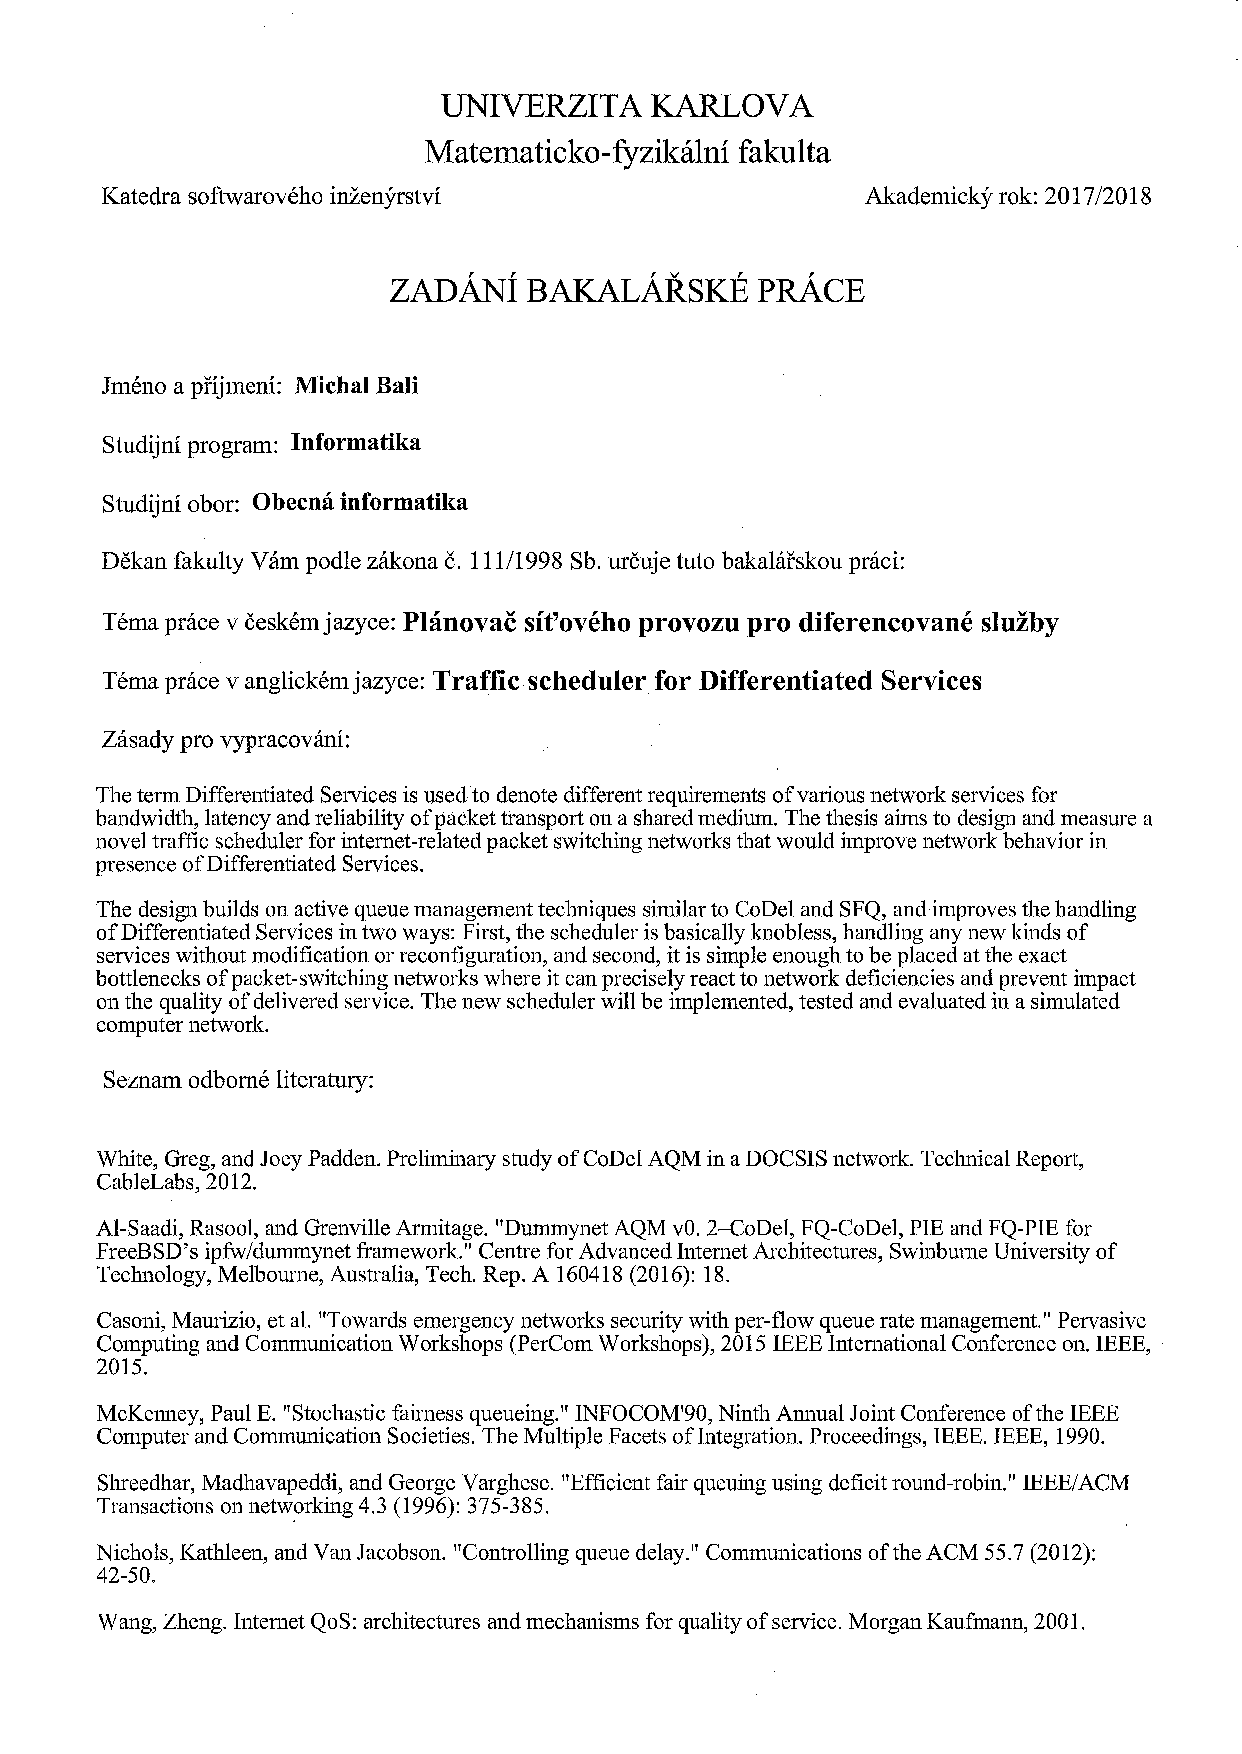
\includepdf[fitpaper=true, pages=-]{assignment.pdf}


%%% Here should be a bound sheet included -- a signed copy of the "bachelor
%%% thesis assignment". This assignment is NOT a part of the electronic
%%% version of the thesis. DO NOT SCAN.

%%% A page with a solemn declaration to the bachelor thesis

\openright
\hypersetup{pageanchor=true}
\pagestyle{plain}
\pagenumbering{roman}
\vglue 0pt plus 1fill

\noindent
I declare that I carried out this bachelor thesis independently, and only with the cited
sources, literature and other professional sources.

\medskip\noindent
I understand that my work relates to the rights and obligations under the Act No.~121/2000 Sb.,
the Copyright Act, as amended, in particular the fact that the Charles
University has the right to conclude a license agreement on the use of this
work as a school work pursuant to Section 60 subsection 1 of the Copyright Act.

\vspace{10mm}

\hbox{\hbox to 0.5\hsize{%
In Prague, date 19.7.2018	% FIXME!
\hss}\hbox to 0.5\hsize{%
signature of the author
\hss}}

\vspace{20mm}
\newpage

%%% Mandatory information page of the thesis

\openright

\vbox to 0.5\vsize{
\setlength\parindent{0mm}
\setlength\parskip{5mm}

Title:
\ThesisTitle

Author:
\ThesisAuthor

\DeptType:
\Department

Supervisor:
\Supervisor, \SupervisorsDepartment

Abstract:
\Abstract

Keywords:
\Keywords

\XX{tady ten template trochu nevychytali, ty keywordy sem asi bude nejlepsi opsat a oddelit carkou rucne, at to dava smysl}

\vss}

\newpage

%%% Dedication

\openright

\noindent
\Dedication

\newpage

\openright
\pagestyle{plain}
\pagenumbering{arabic}
\setcounter{page}{1}


%%% A page with automatically generated table of contents of the bachelor thesis

\tableofcontents

%%% Each chapter is kept in a separate file
\chapter*{Introduction}
\addcontentsline{toc}{chapter}{Introduction}

A traffic scheduler determines when, if and in what order packets leave device. Although a traffic scheduler is present in every device connected to the Internet, it is more important in routers, which handle much more traffic. It has critical impact on performance of packet-switched networks, which naturally makes it an object of interest of Internet Service Providers (ISP).  Not only do they need good physical infrastructure, they also need traffic scheduling to maximize network utilisation and ensure fairness among all clients and overall quality of service. Especially the QoS is provided by differentiating services, since individual services have different requirements for network resources.

ISPs often use traffic schedulers like HTB or HFSC in this situation. They allocate bandwidth to services exactly as the user needs. However, their robustness predetermines them for usage at the edges of networks, because it is impossible for the network administrators to figure out the right configuration for each node. Unfortunately, that is not a desired characteristics, since such schedulers do not have information about the inner nodes and thus cannot react to network deficiencies.

In this thesis, we design a traffic scheduler simple enough to be placed at the exact bottlenecks of networks where it can precisely react to network problems and prevent impact on the quality of delivered service. Priority class is only represented by one number, opposed to hierarchical structure or service curves that apply to HTB and HFSC. The only configuration an user has to provide is a packet classifier. We build on previous research in the area --- the design combines ideas of Controlled Delay (CoDel) and Stochastic Fair Queueing (SFQ) and uses Deficit Round-robin to prioritize more important traffic classes. 


\section*{Related Work}


\section*{Layout of this Thesis}



\chapter{Traffic scheduling}
\label{chap:gf}
%trosku este prepisat tento uvod
One of the pieces of puzzle that make the Internet and generally packet-switched networks work is traffic scheduling. It lies between the second and the~third layer of OSI (or between link and internet layer of the TCP/IP). That means its turn in each single router comes after the network layer did its job: it \XX{determined the packet's next hop and particularly the link,} through which the device is going to transmit the packet. Before the device hands it over to the data link layer and actually sends it, it waits in a buffer. The buffer is needed because of asynchronism of packet-switched networks (further reasons why buffers are needed are discussed in \autoref{chap:bb}).

A traffic scheduler manages the sequence of packets that flow through a device. Most of all, traffic scheduler chooses which packet is going to be transmitted next from the packets that are buffered in the device. Each traffic scheduler has to handle two basic routines: enqueue and dequeue. Enqueue adds a packet to the scheduler and dequeue returns the next packet to transmit.

The natural simplest traffic scheduler is a FIFO queue --- the packets are transmitted by the order of their arrival. In traffic scheduling context, the queue is often referred to as first-come first-serve (FCFS) queue. However, as shown throughout this chapter, problems arise from using such simple solution, that must be solved by using more sophisticated methods instead.

Traffic scheduling severely affects overall performance of networks and particularly the Internet. Because of the universal Internet availability, ever-rising number of services now utilizes the internet protocol, instead of using traditional transfer media (e.g. IPTV, VoIP, teleconferencing). This results in more pressure on maintaining acceptable quality of service (QoS).

The term quality of service is used to denote overall performance of the Internet. There are a few measurable qualities, that are considered to represent QoS well. They are also used to measure performance of traffic schedulers:
\begin{itemize}
	\item Throughput --- the bit rate --- number of bits that are transmitted per second
	\item Packet loss --- ratio of packets, that never reach their destination to all packets.
	%\item Packet errors --- a packet error happens, when the delivered packet is different than the sent packet.
	%packet error nesuvisi s traffis schedulingom, nevidim dovod preco ho spominat.
	\item Delay --- time that elapses between packet sending and receiving.
	\item Jitter --- variance in delay of consecutive packets.
\end{itemize}

Various qualities may be required for different services. Voice over Internet Protocol (VoIP), which allows users to to phone each other over the IP requires small packet delay, packet loss and jitter. Internet protocol television (IPTV) additionally requires sufficient throughput. On the other hand, e-mail does have little requirements whatsoever. Table \ref{tab:QoS} shows different services and their QoS requirements \cite{Tanenbaum:2002:CN:572404}.

\begin{table}
	\caption{Stringency of services’ quality-of-service requirements.}
	
	\label{tab:QoS}
	\centering
	\resizebox{\columnwidth}{!}{%
		\begin{tabular}{@{}lllll@{}}
			\toprule
			Service                        & Throughput & Delay  & Jitter & Loss   \\ \midrule
			E-mail                         & Low        & Low    & Low    & Medium \\
			File sharing (e.g. FTP)        & High       & Low    & Low    & Medium \\
			Web access (e.g. HTTP)         & Medium     & Medium & Low    & Medium \\
			Remote login (e.g. SSH)        & Low        & Medium & Medium & Medium \\
			Audio on demand (e.g. Spotify) & Low        & Low    & High   & Low    \\
			Video on demand (e.g. YouTube) & High       & Low    & High   & Low    \\
			Telephony (e.g. VoIP)          & Low        & High   & High   & Low    \\
			Videoconferencing (e.g. Skype) & High       & High   & High   & Low    \\ \bottomrule
		\end{tabular}
	}
\end{table}


There is a wide range of requirements an ideal traffic scheduler should satisfy. These include avoiding poor performance and other negative phenomena observed in networks and enforcing fairness for all applications (users). Internet service providers use scheduling to define the shape of traffic provided to customers. Researchers have realised the potential of a traffic scheduler years ago and this chapter offers a summary of basic concepts used in the area.



\section{Bufferbloat}
\label{chap:bb}

In gateways of packet-switched networks, short-term differences between arrival and departure rate occur naturally as a result of network multiplexing and applications' behaviour. To balance these bursts, gateways use buffers --- a limited amount of memory, that stores packets, that were received and wait to be forwarded by another link. Traffic schedulers organise the packets in the buffers. In the following paragraphs, we demonstrate the negative effects of using traffic scheduler as simple as FIFO queue.


If the buffer in a device is big enough, every time an outgoing link asks for the next packet, there in one available in the device regardles of differences in packets arrival and departure rate. That is desirable, because the throughput is maximized. Without buffers, the gateway has no place to store incoming packets and thus has to drop them, which decreases throughput.

Even though it may seem that bigger buffers are better, it is not true --- the more packets are in a queue, the longer packets stay in it and the longer it takes to be forwarded, which increases delay. Unfortunately, queues in modern networks tend to fill up and stay 'bloated' \cite{Gettys:2012:BDB:2063176.2063196} --- some amount of packets always stays in the queue (it never becomes empty), even if there are no incoming bursts to balance. This negative phenomenon of constantly full buffers is referred to as bufferbloat. It occupies precious space in buffers and pointlessly increases delay of packets.

\begin{figure}
	\centering
	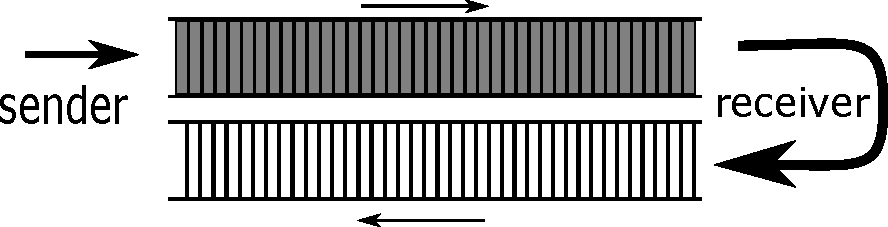
\includegraphics[width=137mm]{drawings/tcp_no_bottleneck}
	\caption{TCP without bottleneck. The grey rectangles are packets. Horizontal dimension is time, vertical is bandwidth. That means the area of rectangle is size of packet.}
	\label{fig01:no_bottle}
\end{figure}

To understand why queues become bloated, let's take a look at Transmission Control Protocol (TCP) \cite{rfc793}, which is currently the most widely used layer 4 protocol. It achieves its reliability with the following policy: After a packet is transmitted, the receiver sends an ACK packet back to sender, to let him know which packets were successfully received, and which packets must the sender resend. Waiting for ACK after each packet would provide miserable throughput and most of the time both sides would wait for single packet. Instead, the sender goes ahead and transmits packets without getting ACKs on previous ones. This fills the whole route, so at all times one packet is being sent, and one packet is being received. The ACKs that come back retain the same spacing. The situation is displayed in Figure \ref{fig01:no_bottle}.

Figure \ref{fig01:no_bottle} shows connection with constant bandwidth along whole path, which is rarely the case in today's Internet. Typical path between the communicants consists of many hops with links of different bandwidth. That means somewhere must be a bottleneck - a link with lowest bandwidth. If the sender transmitted at the rate of the adjacent link, the network would become congested. The bottleneck link would not be able to forward all the incoming traffic, its buffer would fill, and the rest of the arriving packets would be dropped. That actually induces even more traffic, because sender would try to resend the dropped packets.


TCP must limit the upstream rate. In ideal case, it would work at the rate of the slowest link. However, the sender does not have any information about bottleneck whatsoever. Thus, TCP uses congestion window: it is amount of bytes TCP can send without receiving an ACK. When an ACK is received, it frees space in congestion window, and TCP may permit sending the next packet, filling the window again. The sender receives the first ACK after round trip time (RTT) - the time it takes to transmit a packet through path sender-receiver-sender.

To maximize throughput, size of congestion window should be at least the (bottleneck) bandwidth-delay product (product of bandwidth and RTT) bytes. In this case, the sender fills the pipe with packets just before it receives the first ACK and is allowed to send the following packets. On the other hand, if the congestion window exceeds the bandwidth-delay product, the excessive packets stay in queues along the path and cause delay. 

One of reasons of bufferbloat is mismatch between congestion window and actual RTT \cite{CoDel}. In reality, estimating the window size is difficult. Always-changing network load affect both RTT and bandwidth, paths change thanks to rerouteing. Buffers can really only be measured at the bottleneck and even there it is hard to differentiate between useful and useless buffers that only cause delay.

\begin{figure}
	\centering
	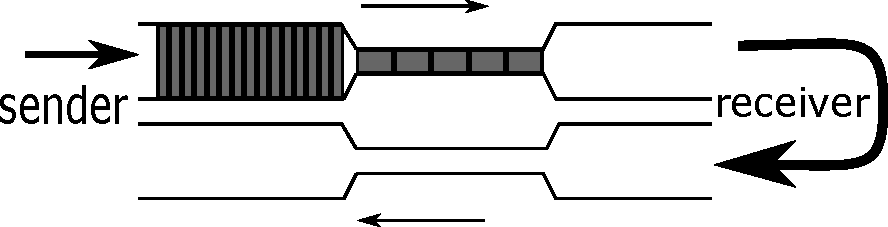
\includegraphics[width=137mm]{drawings/tcp_bottleneck_1}
	\caption{Start of a TCP communication.}
	
	\label{fig02:bottle_1}
\end{figure}


We will take a look at an example to demonstrate that we can observe bufferbloat even in simple situations. Figure \ref{fig02:bottle_1} shows a starting TCP communication. The illustrated network consists of 3 subnetworks. The left and the right have bandwidth 30 Mb/s, the middle one has 10 Mb/s. One packet has 30kb. The TCP Congestion window is 20 packets. The sender starts by transmitting whole window of packets back to back. They arrive at edge of the bottleneck network and get enqueued there, because of the bandwidth difference between left and middle subnetworks. A packet arrives from the left network every 1 ms, but only every 3 ms is one dequeued. At the right side, they retain spacing given by bottleneck as shown in Figure \ref{fig03:bottle_2}. The receiver turns incoming packets into ACKs with the same spacing. The sender then sends one packet of data for each ACK it gets.

This way, after one RTT, the whole connection gets into state of equilibrium. The bottleneck is fully utilized, so the throughput is as high as possible. However, the queue at the middle network never gets empty. At first, it has to hold the burst of the whole congestion window. Once all 20 packets are sent, 14 of them are waiting in the queue, 6 are already forwarded towards the middle network. Then, no packets are enqueued, and every 3 ms one is dequeued. Until one RTT passes, first ACK is delivered, and next packet is sent into left network. After that, one packet arrives and one leaves every 3 ms. 5 packets stay there and every one of them waits long 15 milliseconds. Also, they block buffer space other connections could use. 

\begin{figure}
	\centering
	\includegraphics[width=137mm]{drawings/tcp_bottleneck_2}
	\caption{TCP after one RTT}
	
	\label{fig03:bottle_2}
\end{figure}

The reason why the packets stay in the buffer in Figure \ref{fig03:bottle_2} is that the congestion window is set to 5 more packets than the bandwidth-delay product. Determining the size of the congestion window is not an easy task. At start of TCP, slow start algorithm \cite{Jacobson:1988:CAC:52324.52356} is used to determine the size of congestion window. It grows exponentially, increasing size of the window with each ACK received, until a threshold is reached or a packet is dropped. After that, congestion avoidance takes over to maintain it. Over the years of TCP in service, many variants were introduced. Currently, CUBIC \cite{CUBIC} is used widely. 

The congestion windows are managed by the TCP endpoints, while congestion and bufferbloat takes place in gateways along the path. There is no direct communication channel between them. When the buffer becomes full, the next packets must be dropped simply because there is no room for them. When TCP does not receive an ACK, it the congestion avoidance algorithm reduces the window and slows down.

Explicit Congestion Notification (ECN) \cite{rfc3168:ECN} is a protocol used by routers along network communication path to notify the endpoints that they should slow down, because there is ongoing congestion. There are 2 bits reserved for ECN directly in the IP header. It gives the routers ability to notify endpoints by marking packets instead of dropping them. Both sides have to support ECN - the receiver has to read the 2 bits and send ACK with the same bits back. The sender then may react like the ACK does not arrive at all. In May 2017, 70 \% of popular websites provided passive support for ECN\cite{ECN:proceedings}.

This all indicates that simple tail drop queues that drop packets only when they are full may be suboptimal for internet usage, and can be superseded by more sophisticated queueing algorithms in the gateways. The algorithms involve counter-intuitive idea of dropping perfectly good packets even if buffer is not full yet. But the drop indicates a problem, while still having room for balancing bursts. This approach is called Active Queue Management (AQM), and is recommended to use throughout the Internet. In the following sections, we describe basic AQM algorithms and concepts.

\subsection{Random Early Detection}

\begin{figure}
	\centering
	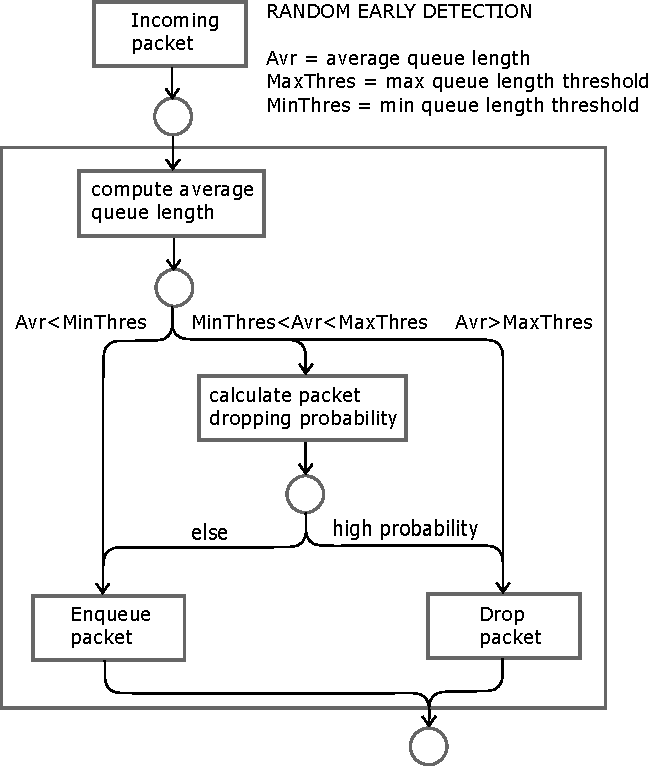
\includegraphics[width=137mm]{drawings/RED}
	\caption{The Random Early Drop algorithm (Image taken from wikipedia \cite{RED:picture}) }
	
	\label{fig04:RED}
\end{figure}

In 1993, Sally Floyd and Van Jacobson introduced Random Early Drop (RED) \cite{Floyd:1993:RED:169931.169935}. It monitored the average length of queue. Based on the average, it may drop (mark) incoming packet with certain (possibly 100 \%) probability, which is function of average. It addressed congestion avoidance problem as well as TCP synchronization problem, that were encountered using tail drop. However, it had quite a few parameters, which have to be set differently in various networks. Without this tuning, it functioned poorly, which led to general reluctance of deployment, although it was recommended by Internet Engineering Task Force \cite{rfc2309} in 1998.

To determine the average of time packets spend in queue, RED uses exponential weighted moving average:
\[
\text{\emph{avg}} := (1 - \textsc{w}_q)\text{\emph{avg}}+\textsc{w}_qq.
\]
$q$ is number of packets in the queue and $\textsc{w}_q$ is parameter of RED that represents degree of weighting decrease, or how much the average responds to new packets and how much weight have the past states. Too high $\textsc{w}_q$ would mean bias against short bursts. With lower $\textsc{w}_q$, the average is more fluid and queue responds to congestion slower.

At each enqueue, the \emph{avg} is compared to two parameters \textsc{MinThres} and \textsc{MaxThres}, as shows Figure \ref{fig04:RED}. If it is lower than \textsc{MinThres}, packet is just enqueued as is. If $avg$ is higher than \textsc{MaxThres}, the packet is marked (dropped). This ensures that if endpoints respond to the marking properly, or packets are actually dropped, the number of packets in queue will not exceed the maximum for long.

If $avg$ is between the thresholds \textsc{MinThres} and \textsc{MaxThres}, the packet is marked (dropped) with probability $p_a$, that is function of the average and number of packets since the last drop. Let $p_b$ be linear function of $avg$ that varies from 0 to $\textsc{Max}_p$ ($\textsc{Max}_\textsc{p}$ is parameter of RED):
\[
  p_b = \textsc{Max}_\textsc{p} \frac{(avg - \textsc{MinThres})}{\textsc{MaxThres} - \textsc{MinThres}}.
\]
Further, the final marking probability $p_a$ depends on when was the last packet marked (dropped):
\[
p_a = \frac{p_b}{1-count \cdot p_b},
\]
where $count$ is number of packets that were enqueued since the last mark (drop). This ensures, that dropped packets will never be too far, nor too close to each other\cite[Section 7]{Floyd:1993:RED:169931.169935}.

RED has also the option to work based on number of bytes in the buffer instead the number of packets. In this case:
\begin{align*}
p_x &= \textsc{Max}_\textsc{p} \frac{(avg - \textsc{MinThres})}{\textsc{MaxThres} - \textsc{MinThres}}.\\
p_b &= p_x \frac{\text{\emph{size}}_{packet}}{\text{\emph{size}}_{max}},\\
p_a &= \frac{p_b}{1-\text{\emph{count}} \cdot p_b},
\end{align*}

where $\text{\emph{size}}_{packet}$ is size of the packet being enqueued and $\text{\emph{size}}_{\textsc{max}}$ is maximum size of packet. This way, large packets are more likely to get marked, and the probability corresponds more precisely to actual time that the packets spend in the queue.

%!!!!!!!!!!!!!!!!!!je v pohode tam dat takyto odstavec o ktorom neviem vela?? ---vicemene jo, mas k tomu citace. Je vhodny dat tam nejaky varianty "other" a "we do not discuss this here" aby bylo jasny ze se tomu nechces venovat.
Over the years, several variants of RED have been introduced. With Weighted RED, different packets have different probability functions for different classes of traffic (classified for example by DSCP). Adaptive RED \cite{Floyd01adaptivered:} tunes the RED algorithm to remove sensitivity to some of the parameters. Robust RED \cite{RRED} was proposed to counter low-rate Denial-of-Service attacks.


\subsection{CoDel}
\label{CoDel}
In 2012, Jacobson and Nichols introduced Controlled Delay (CoDel) algorithm \cite{CoDel}. Their AQM uses local minimum waiting time of packets in queue as indication of bufferbloat. It works only with sojourn time --- the time packets spend in queue. That implies it is independent of bandwidths of adjacent links --- if it is deployed in a backbone with 10 Gbps bandwidth, acceptable queue will be 6.25MB big. On the other hand, on an example slow 10 Mbps link, the corresponding acceptable buffer is only 6.25 kB. CoDel measures the time packets spend in queue and if it exceeds a threshold for a longer uninterrupted time, it starts to drop packets.

CoDel has 2 parameters:
\begin{itemize}
	\item \textsc{Target} is the target delay CoDel tries to keep.
	\item \textsc{Interval} sets period of time for which it is OK to exceed \textsc{Target}.
\end{itemize}
With these parameters, CoDel drops packets if they spend more than \textsc{Target} time in the queue for more than \textsc{Interval} time.

CoDel works in following way: every time a packet arrives, a time stamp is tagged to it. At dequeue, CoDel looks how long was the dequeued packet in the queue. If packets have exceeded the $Target$ time for at least $Interval$, CoDel enters dropping state. In this state, packets are dropped at an increasing rate until the sojourn time of packets at front is lower than $Target$. After each drop, the next drop time is calculated as follows:
\[
  DropInterval = \frac{Interval}{\sqrt{count}},
\]
where count is the number of packets dropped since dropping state entry and DropInterval is the time after the next packet will be dropped.

\todo{Tady bych ocekaval normalni algorithm listing s pseudokodem pro enqueue/dequeue.}

\todo{Oponentova otazka: Proc je tam ta odmocnina? Je za tim trochu matematiky diky ktery to TCPckum ``akorat'' rekne o kolik maj zpomalit. Opsat tu matematiku z paperu by bylo fajn.}
 
CoDel and RED both address\XX{ed} the bufferbloat problem and both manag\XX{ed} to mitigate the problem at the very least. CoDel superseded RED by its easiness to deploy. However, both algorithms work above a single FIFO queue, which is their limitation especially if multiple non-cooperating traffic streams try to use this single queue at once. The next section shows how traffic scheduling may benefit from using multiple queues in parallel.

\section{Fair queueing}

Research shows \todo{`research shows' potrebuje citaci!} that simple first-come, first-serve (FCFS) scheduling does not treat all network users fairly in all situations. In many cases, we want to ensure that every user of a network is provided with the same quality of service. Further, it is beneficial if scheduling separates well and ill-behaved users, so that only the latter experience consequences of their behaviour. Set of \todo{AQM} algorithms that enable this is called fair queueing.

In many of the proposed solutions, fairness is achieved by adding firewalls \todo{definice firewallu? mozna chces pouzit uplne jiny slovo} between different streams of packets traversing network, or flows. We use definition from \cite{Zhang:1990:VCN:99517.99525}. A flow has two properties:
\begin{itemize}
	\item A flow is a stream of packets that traverses the same route from the source to the destination and requires the same grade of service at each router or gateway in the path.
	\item In addition, every packet can be uniquely assigned to a flow using prespecified fields in the packet header.
\end{itemize}
 
\begin{figure}
	\centering
	\includegraphics[width=137mm]{drawings/parking_lot}
	\caption{The parking lot problem. \XX{v captionu je potreba vysvetlit co znamenaj ty cisla}}
	
	\label{fig05:ParkingLot}
\end{figure}

One of the issues addressed by fair queueing is the parking lot problem. Typically, routers accomplish some amount of fairness by giving fair access to traffic coming from different input links. However, this approach is not fair to all flows. Consider network displayed in Figure \ref{fig05:ParkingLot}. Gateway G1 treats both flows F1 and F2 equally, thus both flows occupy half of link G1--G2. G2 does the same, it gives half of the bandwidth to flow 3 and second half to the traffic from link G1--G2. However, from perspective of flows, F1 and F2 have only 1/4 of the bandwidth while F3 has half of the bandwidth. In the outcoming link of G3, situation is the same and F1 only has one 1/8 of the bandwidth. In other words, portion of bandwidth allocated to flow drops exponentially with number of hops it gets through.

Second issue is related to behaviour of the users themselves. In gateways working on FCFS basis, misbehaving user that sends more traffic than others, and does not slow down on packet drops, may actually get bigger portion of bandwidth than well behaving users. Consider a router with several users connected on LAN, one of them is ill-behaved and generates traffic that by itself exceeds routers out--link. The rest of users detect congestion and slow down, resulting in leaving even bigger proportion of the bandwidth to the bad user. Furthermore, delay discussed in section \ref{chap:bb} is shared among all users and if one bloats the buffer, the others experience consequences too.

To battle these problems, Nagle \cite{Nagle:FQ} proposed to use one FCFS queue per one flow encountered by the gateway. At enqueue, router finds the right queue based on the IP header. Queues are dequeued in a round-robin fashion --- the queues take turns in fixed order. There is a list of all queues and at each dequeue gateway transmits the first packet of the first queue in the list. Then, the first queue is taken from the front and put in the back of the list. In other words, at each dequeue, the queue (flow) that was not served for the longest time is chosen (with the exception of brand new queues).

%flow stealing

This solves both of mentioned problems, maintaining separate queue for each flow requires that the gateway to be able to map from flow identifiactor (for example source-destination address pair, ports and protocol may be considered too) to corresponding queue at each dequeue. This can be easily implemented in $O(log n)$ \todo{tohle si prosim vsude predelej na $\mathcal{O}(\log n)$.}, where n is number of queues, however that is not fast enough for simple routers with ever-rising bandwidths. McKenney discusses several possible implementations in \cite[Section 2]{SFQ}.

Nagle's original algorithm has yet another flaw --- it doesn't take packet size into consideration. So if flow A sends only 100B packets, and flow B sends 500B packets, flow B gets five times more bandwidth. To address the flaw,  Demers et al. devised an ideal algorithm called bit-by-bit round-robin (BR) \cite{demers1989analysis}. It simulates that each queue sends one bit at a time in round-robin fashion. Based on this simulation, it computes time $t$ the whole packet would leave its queue. Then, BR inserts the packet in a queue sorted by $t$. Unfortunately, the best known algorithms that insert into sorted queue require $O(log n)$ time, where n is the number of flows (since at most one packet from each flow needs to be in the priority queue at the same time).

Although the Nagle's FQ algorithm was perfected to be truly fair, it requires too much resources. Following algorithms have O(1) complexity, while being only slightly less fair.


\subsection{Stochastic Fairness Queueing}
%aspon jednu figure bud z FQ alebo SFQ?

SFQ was proposed by McKenney \cite{SFQ} to address the inefficiencies of Nagle’s algorithm. It uses hashing to determine the flow each packet belongs to. Although one would normally require one queue for every flow and thus use hashing with chaining, McKenney suggests using considerably less queues and allow collision. This guarantees $O(1)$ queue determination. The disadvantage is that some flows may collide, end up in the same queue, and thus be treated unfairly. However, if the number of queues is sufficiently larger than the number of active flows, probability of unfairness is low. To further beat this disadvantage, SFQ changes the hashing periodically (e.g. every 10 seconds) by varying salt of the hash function.

SFQ services its queues in round-robin fashion, without taking packet lengths into consideration, so it is unfair, if average packet size vary in the flows.

SFQ uses bufferstealing: When there is no more space in the buffer, a packet is dropped from the queue with the highest number of packets instead of dropping packet being enqueued. To implement this in O(1), McKenney suggests bucket sorting technique: there is an array indexed by number of packets. In $i$-th field of the array, there is a list of all queues that contain $i$ packets.

McKenney's scheme is valuable for bufferstealing and stochastic approach, however does nothing about unfairness caused by flows having different size of packets.

\subsection{Deficit round-robin}
\label{DRR}
Deficit round-robin \cite{EffDRR} is an algorithm that extends SFQ and takes packet length into consideration, so every flow gets the same bandwidth in the long term regardless of its packet characteristics. For each queue, it uses deficit counter that counts how many bytes were dequeued from the queue. If a packet can not be sent because it is too big, remaining bytes in the counter transfer to the next round. It still requires only $O(1)$ time for all the operations.

For each flow, DRR needs parameter $Q_i$, where $i$ is flow number. $Q_i$ roughly specifies how many bytes DRR can send from flow $i$. If $Q_i = Q_j$ for all $i$ and $j$, all queues get the same share of the bandwidth, and thus is fair. If $Q_i$ is twice $Q_j$, $i$-th to $j$-th bandwidth will be in ration $2:1$.

Enqueue is done in the SFQ--way: DRR chooses queue based on hash of certain IP header fields. It keeps list of active queues and works in $O(1)$. When the buffer is full, packet is dropped from the fullest queue instead of dropping the incoming one.

The novelty of DRR lies in modified round-robin. There is a state variable $DC_i$ for each flow. The $DC_i$ is set to $Q_i$. At each round, DRR sends at most $DC_i$ bytes. Once sending next packet would break this rule, DRR puts queue  at the back of active queues list and sets $DC_i$ :
\[
  DC_i = DC_i - b_{sent} + Q_i.
\]
$b_{sent}$ is number of bytes sent that round from queue i --- that is subtracted from $DC_i$. Further, DRR replenishes the deficit counter, so it may send packets in the next round. If there are no packets in queue left, it is deactivated instead of putting it in the back.

\begin{algorithm}[t]
	\caption{DRR queueing algorithm}
	\label{alg01:DRR_deq}
	\begin{algorithmic}
	\Function{enqueue}{}
		\State \Return \XX{TODO}
	\EndFunction
	\Function{dequeue}{}
		\While{true}
			\State F $\leftarrow$ pop(ActiveQueues);
			\If {empty(F)}
				\State Deactivate(F)
			\ElsIf{F.DC \textgreater~head(F).PacketSize}
				
					\State {F.DC $\leftarrow$ F.DC - head(F).PacketSize}
					\State \Return pop(F)
			\Else \Comment{The packet is bigger than DC}
				\State F.DC $\leftarrow$ F.DC + Q
				\State push(ActiveQueues, F)
			\EndIf
		\EndWhile
	\EndFunction
	\end{algorithmic}
\end{algorithm}

Although DRR may not send exactly the same amount of bytes each round, it becomes fair (if all $Q_i$ are equal) in several rounds time, because every round, all that remains in $DC_i$ from the previous round transfers to the next. Thus, any unfairness caused by atomicity of packets are smoothed over time.

%analyza??
\todo{je potreba odkazat refem algoritmus z textu}

\subsection{Flow Queue CoDel}

\begin{figure}
	\centering
	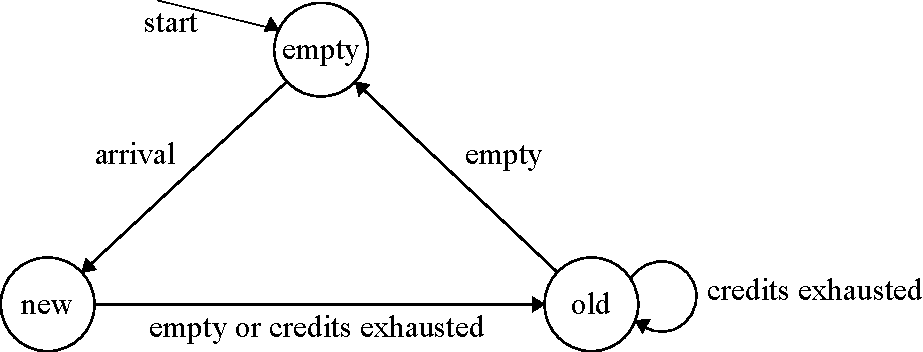
\includegraphics[width=137mm]{drawings/fq_codel}
	\caption{FQ-CoDel state-machine. \XX{Sipku vlevo nahore by to chtelo okomentovat jako `start' protoze takhle vypada trochu jako enqueue.}}
	\label{fig06:fqcodel}
\end{figure}

Flow Queue CoDel \cite{fq_codel} is a traffic scheduler that combines ideas of SFQ and DRR with CoDel bufferbloat battling capability. It uses modified DRR and replaces FCFS queues for flows with CoDel queues. Currently, several linux distributions as well as systemd use FQ CoDel as the default traffic control.

In the context of FQ CoDel, term credits is used instead of deficit counter. However, the two denote the same state variable.

FQ CoDel processes the flows in the DRR fashion, however it divides active queues into two groups: new and old. The new ones are prioritized: packet is never dequeued from an old flow, if list of new queues is not empty. An empty queue becomes new, when a packet is enqueued to it. New queue becomes old (it is pushed at the back of old flows list), if it becomes empty, or its credits ($DC$) are exhausted. An old queue becomes empty, if there are no packets left in it. So every flow has its life cycle in this order: it is first empty, then new, old and empty again. The state machine is illustrated in Figure \ref{fig06:fqcodel}.

FQ CoDel has parameters $Target$ and $Interval$ that configure the underlying CoDels. Further, there is $Quantum$, that is parallel of DRR's $Q_i$, however $Quantum$ applies to all queues. $Limit$ is the maximum number of packets the scheduler can hold at the same time.

When a packet is enqueued in FQ CoDel, its flow is found based on its IP header in the SFQ fashion. Then, CoDel takes it over - it is timestamped and put in the back. If the flow is empty, it is pushed back into the list of new queues and its credits are set to $Quantum$.

To protect buffer from overload, FQ CoDel keeps track of total packets it is holding. Since a packet is just enqueued, $Limit$ may be exceeded. If it is, the algorithm finds queue with the largest byte count and drops 64 packets from the \textit{front}. Dropping several packets at once amortises the time needed to find the longest queue.

The algorithm does most of the work at dequeue. First, it chooses a flow $F$ to dequeue packet from --- either the head of new queues list, or the head of the old queues list, if the new one is empty. If $F$ has negative credits, it means FQ CoDel already served at least $Quantum$ bytes, and pushes it in the back of the old queues list and starts over with choosing $F$.

Second, it dequeues packet from CoDel of flow $F$. Two things may happen:
\begin{enumerate}
	\item CoDel drops all packets on dequeue --- change state of the flow based on Figure \ref{fig06:fqcodel} and start over.
	\item CoDel returns a packet --- subtract the size of packets from credits of flow $F$ and send the packet away.
\end{enumerate}

FQ CoDel is fast and simple enough to be deployed in ordinary home routers. Furthermore, it combines good characteristics of CoDel and SFQ.

\section{Traffic shaping}

In some applications, perfectly fair queueing (the same bandwidth for all) may not be emphasized\todo{applicable?}. Instead, it is beneficial\XX{,} to give up the best-effort basis in order to maintain good QoS for all users and services in the network, as different services have different needs and different users have different service level agreements. 

Traffic shaping is set of techniques for regulating the average rate and burstiness of a flow of data that enters the network. The customer and ISP agree on certain traffic pattern (or shape) that provider then shall guarantee. ISP tries to suit all application's requirements for QoS. Also, the goal is to describe traffic patterns in a simple and robust way. Traffic shaping provides ISP with the ways to do it. It is also suitable for congestion avoidance, since it controls amount of traffic in network.

%Traffic policing takes care of the opposite aspect of the SLA - limiting the services provided. ISP monitors traffic users generate and if it exceeds the agreed traffic pattern, it may drop packets.

\subsection{Leaky bucket and Token bucket}
\label{token_bucket}
Leaky bucket (first described by Turner in \cite{turner1986new}) and token bucket are two terms used for the same concept, they only use a slightly different analogy with bucket and water/tokens as described in \cite[Section 5.4.2]{Tanenbaum:2002:CN:572404}. However, both schedule packets at constant rate and drop packets, if they flow too fast while allowing certain burstiness.

Both use the same parameters - rate $R$, at which packets leave and size of bucket $B$, also called burst size.

\begin{figure}
	\centering
	\begin{subfigure}{.6\linewidth}
		\centering
		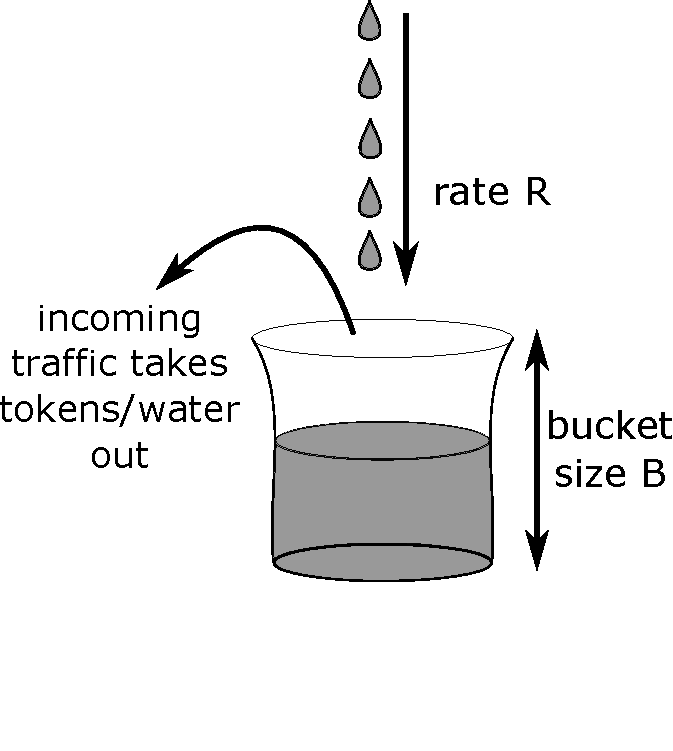
\includegraphics[width=75mm]{drawings/token_bucket}
		\caption{Token bucket}
		\label{fig08:token}
	\end{subfigure}%
	\begin{subfigure}{.4\linewidth}
		\centering
		\includegraphics[width=47mm]{drawings/leaky_bucket}
		\caption{Leaky bucket}
		\label{fig08:leaky}
	\end{subfigure}
	\caption{\XX{sem je potreba napsat nejakej pokec co to vlastne je. Btw myslim ze incoming se pise s jednim M, dve M se davaj do podobnyho slova ktery nejspis nesouvisi.}}
	\label{fig08:token_leaky}
\end{figure}

Illustration of a leaky bucket is in Figure \ref{fig08:leaky}.The algorithm needs a counter variable $C$. If there is any water in the bucket ($C > 0$), it leaks ($C$ decreases) at rate $R$. Every time a packet comes, its size is added to this counter. If $C + PacketSize$ is more than $B$, packet must wait until $C + PacketSize < B$ holds (until enough water leaks) or is dropped. Note, that R is not the same as the output bandwidth. When the bucket is empty, the leaky bucket sends packets as they come until the bucket is filled. 

Token bucket is in Figure \ref{fig08:token}. In this case, algorithm adds tokens to $C$ at rate $R$. Every time a packet passes, it takes tokens equal to its size from the bucket (its packet size is subtracted from $C$), or, if $C - PacketSize < 0$, the packet must wait until enough tokens are in $C$. 

%The general concept is, that there is one bucket for each user.
The concept may be used in two ways --- in the place of scheduler, that actually holds the packets in FCFS queue. Secondly, ISPs can use it in traffic policing, to enforce service level agreement. In that case, token/leaky bucket just manages the buckets based on packets that flow by, and drops them if the buckets are empty/full.

The fundamental feature of the bucket concept is, that it enforces certain bandwidth, while allowing short-term bursts (that are necessary in networks). Let M be maximum output rate in B/s, and t the time between start of burst and dropping (withholding) first packet. Then it holds:
\[
	B + RS = MS,
\]
since water leaks from the bucket even after the burst begins. $B + RS$ is number of bytes bucket permits, $MS$ is the number of bytes output link is able transmit. Thus,
\[
	MaxBurstSize = MS = M\frac{B}{M - R}.
\]

\begin{figure}
	\centering
	\includegraphics[width=137mm]{drawings/tbf}
	\caption{Token bucket filter. Picture taken from wikipedia \cite{TBF:picture}}
	
	\label{fig09:tbf}
\end{figure}

\subsection{Token Bucket Filter}
Token Bucket Filter (TBF) is traffic scheduler implemented in the Linux kernel. It uses the token bucket with FCFS queue. Additionally, it limits peak maximum output rate by adding second small bucket. This bucket is only the size of the maximum transmission unit (MTU), and has the higher configurable peak rate --- TBF never transmits at higher rate that this peak. It prevents the scheduler from taking all the bandwidth of the output link.

It is shown in Figure \ref{fig09:tbf}. TBF enqueues packets into common FCFS queue. It may become full, if number of bytes in it exceeds $Limit$ --- then incoming packet is simply dropped. The dequeue is controlled by two token buckets --- both of them must have enough tokens to allow packet sending. The smaller bucket is size of MTU, $Rate$, $PeakRate$ as well as size of the bigger bucket $Burst$ are parameters of the algorithm.

\subsection{Hierarchical token bucket}
\begin{figure}
	\centering
	\includegraphics[width=137mm]{drawings/hierarchy}
	\caption{Traffic pattern organized in a hierarchy.}
	
	\label{fig10:hierarchy}
\end{figure}
In the area of traffic shaping, it is important to be able to precisely define traffic shape, and to have an algorithm that can follow this definition as precisely as possible. Hierarchic definitions are a natural way to do so. One such hierarchy is shown in Figure \ref{fig10:hierarchy}. It shows a link with 45 Mbps of bandwidth. Two organizations: CUNI and CTU share this link. The first one is guaranteed 25 Mbps and the latter 20 Mbps of the bandwidth. Both organizations then define their internal traffic shape they want to have guaranteed.

Every node is guaranteed to receive \textit{at least} the specified rate at all time. We want the link to be utilized as much as possible at all times. For example, when CUNI only transmits 5 Mbps of video traffic, the excess 3 Mbps may be shared with the rest of classes - first with sibling ones, and if whole CUNI does not generate enough traffic, CTU gets more than the guaranteed 20 Mbps.


Secondly, we need an algorithm, that would enforce the hierarchy. One such algorithm is Hierarchical Token Bucket (HTB) [ref??]. It divides traffic into classes that are further hierarchically grouped in a tree. Classes are divided into 8 levels of priority, which affects delay and distribution of excess resources, but not guaranteed rate. At actual dequeue, HTB uses deficit round-robin to serve all classes of the same priority, while conforming to token bucket limitations.

Every node of the tree takes several parameters:
\begin{itemize}
	\item priority --- classes with higher priority are served first. 0 is the highest priority and 8 is the lowest.
	\item rate --- guaranteed rate the class gets.
	\item ceil --- maximum rate the class can get.
	\item burst --- size of the main bucket (see \ref{token_bucket}).
	\item cburst --- size of the ceil (peak) bucket, should be set small, like average size of packet.
\end{itemize}

There are two token buckets in each class, one with size $burst$ and rate $rate$, the second determines maximum rate, has size $cburst$ and rate $ceil$. The main idea of HTB that allows distribution of excess resources is, that child classes can borrow tokens from their parents, if they have exceeded $rate$ (and do not have any tokens left in the main bucket). They are, however, still limited by $ceil$. According to this, classes can be divided into 3 groups. Then:
\begin{itemize}
	\item Green --- Class has enough tokens (does not exceed $rate$)
	\item Yellow --- Class exceeds $rate$, but does not exceed $ceil$. It may borrow from parent class(es).
	\item Red --- Class exceeds $ceil$, and packets must be backlogged until it gets more tokens (either its own or borrowed).
\end{itemize}


When HTB determines which class to dequeue, it chooses the colour of class first. It serves an yellow class only if there are no green ones. Red classes are never served. Green classes are the ones that do not reach the guaranteed rate yet and thus have highest priority. Next, it filters classes based on priority: HTB never chooses class of priority $i$ if any of the priorities $\left\langle0,i\right)$ are available. If there are more classes of the same priority and color, they are served in round-robin fashion using DRR with the quantums of classes set according to the class $rate$. By default, quantum is 1/10 of $rate$. 

The yellow classes may only borrow from its parent, if it is not red. If it is yellow, it results in recursion --- parent has to borrow tokens from grandparent and so on.

In other words, HTB uses the token bucket hierarchy to mark classes with colour and thus prioritize ones, that have not received $rate$. On the second level, it prioritizes classes with higher priority. On the third level, all classes are equal, thus it uses DRR. On the fourth level, there is usually FCFS queue to buffer the withheld packets. However, in the implementation in the Linux kernel, one may assign any qdisc to each class.

%HFSC --- asi neni potreba, mozna bys moh udelat jen nejakej rychlokapitolu s tim ze "other queueing disciplines" kde rychle zminis HFSC, CBQ, PIE, BLUE, Choke, QFQ a podobny kraviny a nejak rychle to uzavres.
%zaver?

\chapter{Our traffic scheduler}
\label{chap02}
%mby a little intro config (knobless), fast O(1), QoS aware, scheduler in presence of differentiated services. Would run at simple devices
Also, CoDel does not drop packets, if fewer that MTU (Maximum Transmission Unit) worth of bytes is in queue.\todo{tohle je takovej dovetek kterej tam je kvuli work-conservation, to muzes vklidu presunout bud do poznamek nebo do kapitoly o implementace}.


\begin{figure}
	\centering
	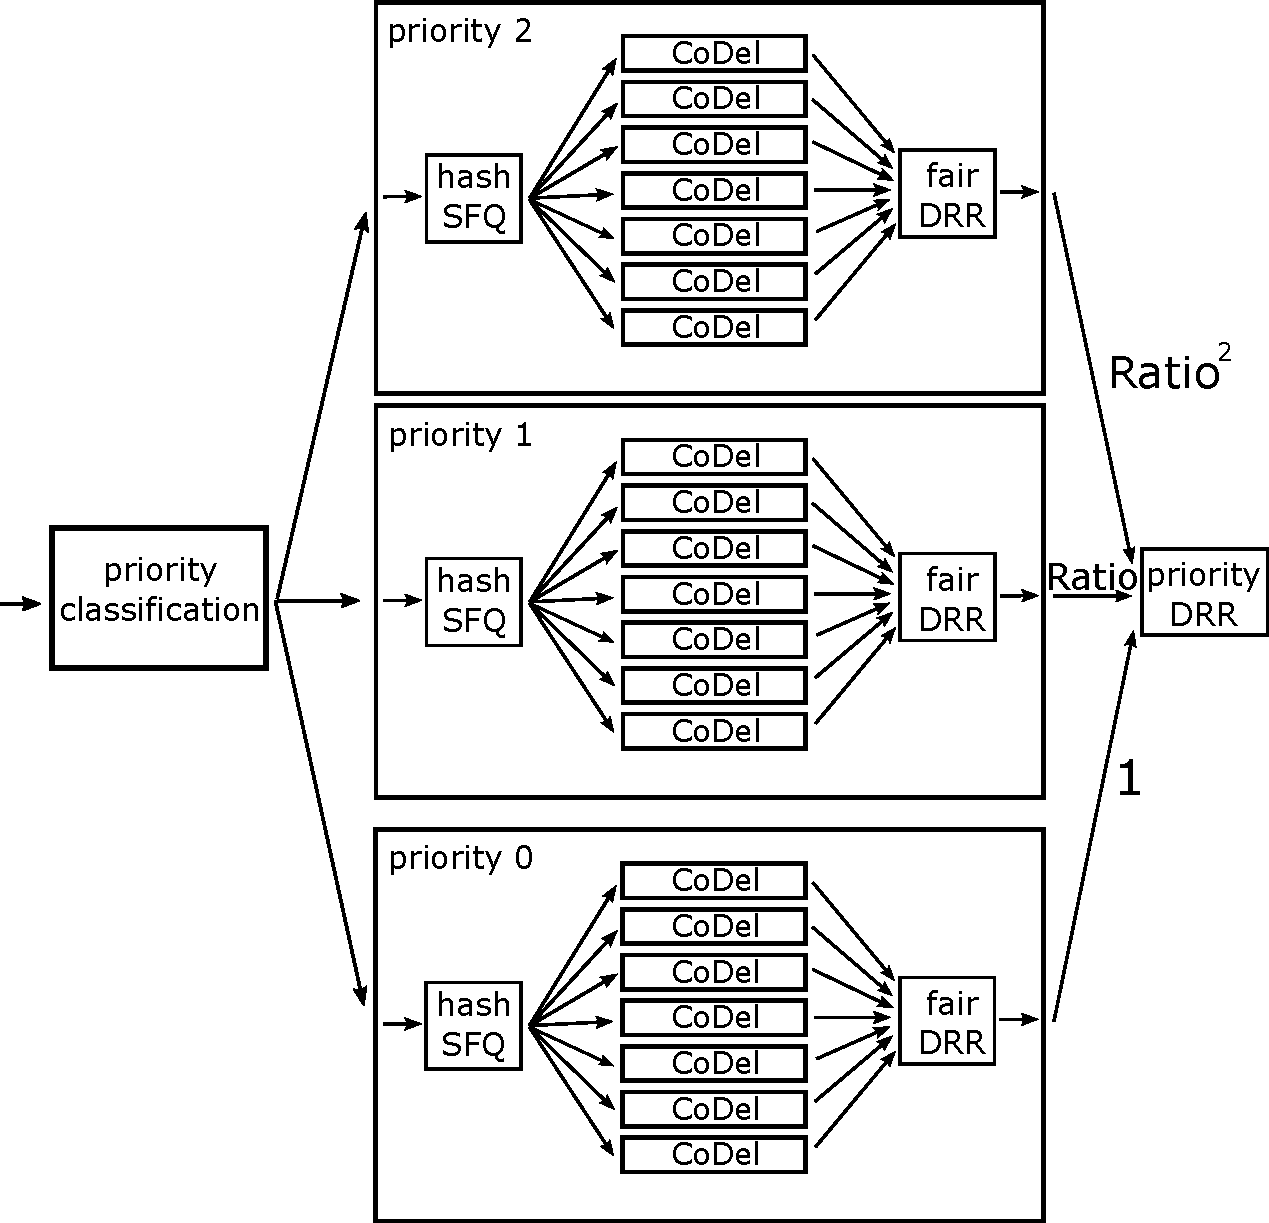
\includegraphics[width=137mm]{drawings/msfc}
	\caption{The MSFC layout}
	\label{fig10:msfc}
\end{figure}

In this thesis, we study traffic scheduler Multilevel stochastic fairness queueing (MSFC) illustrated in \ref{fig10:msfc}. It combines ideas of previous work: CoDel and deficit round-robin, to create traffic scheduler. It uses three-level layout. In the highest level, packets are assigned to priority classes. We use non-fair DRR to prioritize more important traffic. Inside the classes, packets are distributed into flows (based on source and destination IP addresses, ports and protocol) and we use second, independent fair DRR to schedule traffic within the class. Each flow uses CoDel algorithm.

Additionally, it has following parameters:
\begin{itemize}
	\item $Limit$ --- the maximum amount of packets stored in the qdisc.
	\item $Prios$ --- the number of priority classes.
	\item $Flows$ --- the number of queues (CoDels) in each priority class (so there are $Prios*Flows$ total independent CoDels)
	\item $Backlog$ --- the maximum backlogged bytes in an individual CoDel.
	\item $Perturb$ --- number of seconds after flow-classification hash function changes
	\item $Quantum$ --- the quantum parameter of the inner fair DRR (see \ref{DRR})
	\item $Target$ --- target delay parameter for CoDel algorithm (see \ref{CoDel})
	\item $Interval$ --- Interval parameter for CoDel algorithm (see \ref{CoDel})
	\item $Ratio$ --- defines the ratio of bandwidth of two adjacent priority classes. The ratio is enforced by the outer DRR. MSFC uses $Ratio$ to compute quantums of all priority classes. The quantums rise exponentially:
	\[
	Q_p = Quantum \cdot Ratio^p,
	\]
	where $p$ is the priority of class, and $Quantum$ is the parameter for inner DRR.
\end{itemize}
So if there are 3 classes with priorities 0, 1, 2 (like in the Figure \ref{fig10:msfc}), the upstream bandwidth will be distributed in ratio $1:Ratio:Ratio^2$.

Note, that the ratio is independent of the number of flows in each class. Consider two classes with adjacent priorities 0 and 1. Priority 1 class has only one flow backlogged, priority 0 class has 100 flows. The one flow from priority 1 class is guaranteed to receive 2/3 of the bandwidth. The 1/3 is distributed fairly between the remaining 100 flows.

%fq codel -new old distinction vs remembering quantum when deactivating

\section {Implementation}

We have implemented the MSFC algorithm into the Network simulator 3 (ns3) to evaluate in simulated conditions. We also describe existing Linux implementation that can be used for actual deployment in real devices.

\subsection {Linux}
\begin{figure}
	\centering
	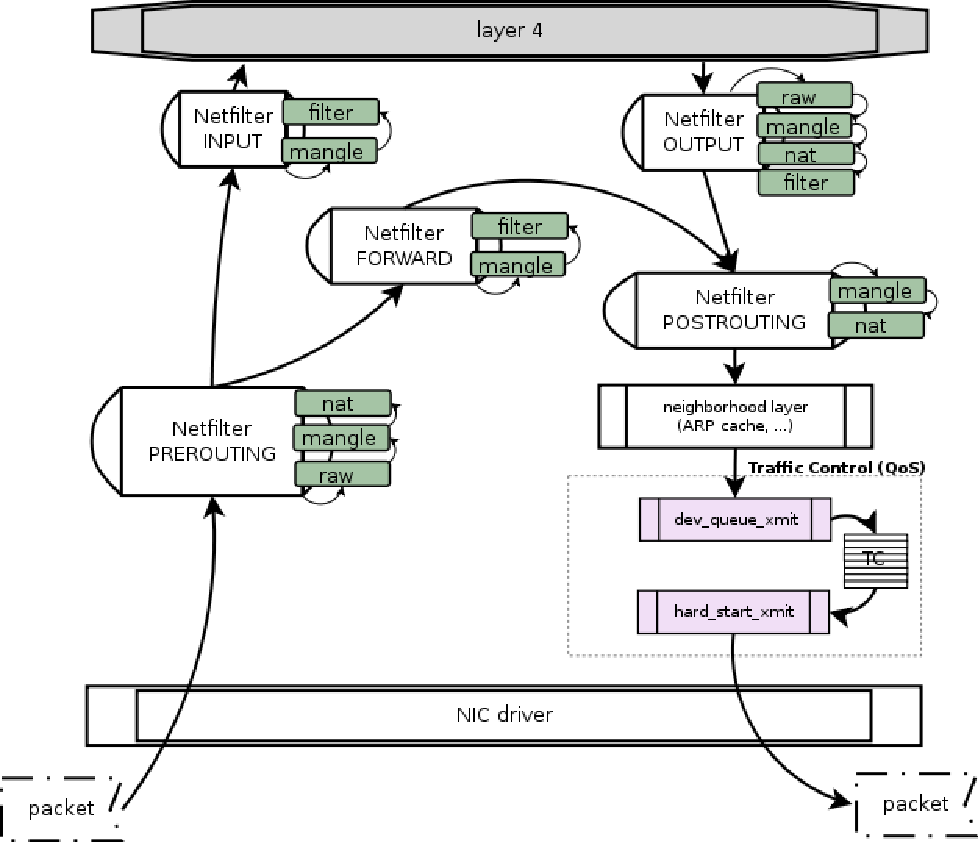
\includegraphics[width=137mm]{drawings/network_stack}
	\caption{Packets traversal through Linux kernel. Picture taken from \cite{linuxCore}}
	\label{fig12:linux}
\end{figure}

To understand the Linux implementation, let us take a look how Linux controls network traffic. The Figure \ref{fig12:linux} shows the context of traffic control in the Linux kernel. It takes place at the bottom of the third (IP) layer, and stores packets that are ready to be handed over to the link layer (realised by Network Interface Card --- NIC).

%The link layer is realised by Network Interface Cards (NIC) in common computers. So when a packet  So the traffic control queue is the place, where 

There are three kinds of objects used in traffic control: qdisc (queuing discipline), class and filter \cite{tc}. Simply put, qdisc is traffic scheduler --- its role is to enqueue packets, store them, and choose an outgoing packet when NIC driver asks for one. Every interface must have at least one qdisc --- root qdisc. It may further contain child classes and each class contains exactly one qdisc. Classless qdiscs comprise only one qdisc object. Filter objects allow packet classifying and policing.

When kernel decides a packet is ready to be sent, it enqueues the packet in root qdisc (that exists in every configuration). If the root qdisc is classful, it may end up in any of its child classes. An arbitrary number of filters may be assigned to every class. When a packet arrives to qdisc with multiple child classes, it calls all the filters one by one, until one of them returns with a verdict. The qdisc then enqueues the packet in child qdisc of the chosen class.

However, the concept of classes and filters is not obligatory to use, it depends on implementation of particular queueing discipline. For example, a classful qdisc may not use filters to classify packet, but use a different method instead (e.g. Type of Service field in IP header). Also qdisc may be classless in relation to Linux kernel, but still use internal 'classes' --- treat different groups of packets differently.

In the kernel, packets are represented by struct sk\_buff (socket buffer). This avoids copying of packets and provides us with attributes like pointer to socket where packet was created, timestamps, length, etc. One of the attributes is (queuing) priority. By default, the kernel sets the priority to value of field Type of Service from packet IP header. However, user may configure the system to change the priority in postrouting mangle phase (see Figure \ref{fig12:linux}) and thus classify packets even before they come to qdisc.

The default qdisc is pfifo\_fast. It is three-band first-come first-serve scheduler. There are 3 independent FIFO queues, one for each priority. Pfifo\_fast classifies packets based on priority attribute of sk\_buff (it takes 4 least significant bits). The dequeue is simple: it iterates dequeues packet from highest priority non-empty FIFO queue.

Every qdisc is connected to the kernel via struct Qdisc\_ops. It defines pointers to methods that the kernel calls to operate the qdisc. Every qdisc then defines variable of type Qdisc\_ops and assigns implementations of corresponding methods to the members of the struct. The most important members are:
\begin{itemize}
	\item enqueue --- Takes sk\_buff argument. It is called every time kernel adds a packet to the qdisc.
	\item dequeue --- Returns dequeued packet.
	\item peek --- Returns packet that the qdisc dequeues next.
	\item init --- Kernel calls it to initialize the qdisc in the beginning of its operation. Here the qdisc may allocate memory and sets its parameters.
	\item destroy --- It is called when operation of the qdisc stops. The qdisc should deallocate all its resources (memory, etc.).
	\item reset --- Kernel calls it to reset the qdisc into the default (empty) state.
\end{itemize}

The Linux implementation follows the 3-level layout of the algorithm. priority class is represented by struct msfc\_prioclass and one CoDel flow by struct msfc\_flow. The amount of memory that the implementation needs is constant throughout the lifetime of qdisc, and it can be computed from parameters $Prios$, $Flows$. MSFC needs an array of priority classes of size $Prios$ and an array of CoDel flows of size $Prios * Flows$. The implementation allocates all the memory in the initialization (msfc\_init) of the qdisc.

The enqueue function needs to determine the right CoDel flow to store the packet. Priority is taken solely from priority attribute of sk\_buff. Then, it uses Jenkins hash implemented in Linux to determine the right flow. The packet enqueued is then put in the back of flow using the pointer to the tail in msfc\_flow. 

The dequeue implements two DRR algorithms and the CoDel algorithm. For each priority class, the quantums are computed during initialization. The qdisc holds pointer to the prioclass that is the next as well as its deficit. The msfc\_prioclass structs handle the state variables of the inner DRRs, which determine the flow from which the packet is dequeued. Finally, CoDel dequeue is used to obtain the packet --- the msfc\_flow struct contains the state of the CoDel algorithm used for the particular flow.

\subsection {ns-3}

Ns-3 (Network Simulator 3) is a discrete-event computer network simulator \cite{ns3}. It provides abstractions of real world objects and devices, and then simulates real (physical) phenomena and technologies as precisely as possible.  It allows us to perform replicable  experiments in a controlled environment that would never be possible in reality.

One of key abstractions of ns-3 is \emph{node}. It represents a network device --- a computer, router, server, etc. Node itself does not have any functionality; It is a container, into which we may install applications, network interfaces and protocols.

NetDevice is abstraction of network interface of a computer. One node may contain more NetDevices, just like common notebook may contain both WiFi and Ethernet interface cards. NetDevices are closely related to channels. A channel represents connection between nodes (more specifically netdevices). For example, it may model something as simple as Ethernet cable, but also complex things like three-dimensional space full of obstructions in case of wifi channel. The simplest channel is point-to-point channel, which connects two netdevices with configured bandwidth and delay.

%seed
%overview how it runs   It simulates all the proceses like real software does, and simulates the fact, that everything takes time in reality using the discrete events. Technically, an event is a timestamp with pointer to function and its parameters. Each event is processed at certain time and may generate additional events at later time. 

\begin{figure}
	\centering
	\includegraphics[width=80mm]{drawings/ns3_internet_stack}
	\captionsetup{justification=centering}
	\caption{Packet traversal through ns3 Internet stack. Picture is based on ns3 documentation \cite[p. 88]{ns3Doc}}
	\label{fig13:ns3}
\end{figure}

This concept of nodes, netdevices and channels works generally for all networks. To simulate the Internet we must install the Internet stack --- set of common protocols that are implemented in every device connected to the Internet. That includes TCP, UDP, IP (v4 or v6) or ARP. The whole ns3 stack is displayed in Figure \ref{fig13:ns3}. Traffic control takes place just before the packet is handed over to NetDevice. However, installing traffic control layer to a node is not mandatory; If none is present, ns-3 sends the packets directly to NetDevice.

The ns-3 traffic control simulates the traffic control objects in the Linux kernel. Qdisc is represented by QueueDisc, class is QueueDiscClass and filter is named QueueDiscFilter. We implemented MSFC as QueueDisc, CoDel flow as QueueDiscClass and we use filters (one for IPv4 and one for IPv6) to hash packet headers to classify them into the CoDel flows.

%The word class is overloaded in the next few paragraphs: one meaning is traffic control class and second is C++ class. We will use

The implementation is as straightforward as possible. We extend the C++ abstract class QueueDisc, the most important methods are again DoDequeue and DoEnqueue. We represent the MSFC priority class by C++ class MsfcPrioClass and one flow is represented by C++ class MsfcFlow. We use the ns-3 implementation of the CoDel algorithm --- there is a CoDel QueueDisc assigned to each MsfcFlow (using general QueueDiscClass mechanism). The actual packets are enqueued in the CoDel QueueDisc.

By default, we determine priority of a packet simply by DSCP field in its IP header. However user can change this easily using ns-3 attribute system by providing a different method that classifies packets. 

The usage of ns-3 CoDel helped us a lot --- we only need to find the right flow during DoEnqueue and then enqueue the packet in the found QueueDisc. First, we determine the enqueuing packet priority to determine the right MsfcPrioClass. The priority classes are organised in a map (pairs priority--MsfcPrioClass). Further, each MsfcPrioClass contains a structure, that maps packet hash (computed by assigned filters) to corresponding MsfcFlow. Finally, we call the Enqueue method of underlying CoDel QueueDisc.

In the dequeue, we implement the two--level DRR. We maintain a list of active priority classes --- the head of the list is the MsfcPrioClass that is the next in the outer DRR. Each MsfcPrioClass holds its deficit and quantum computed based on the priority when the first packet with the particular priority is enqueued. If the priority class does not have any packets, we deactivate it and remove from the list. We activate it again when a packet of the priority is enqueued.  

The same applies to flows within each priority class. Each MsfcPrioClass contains a list of active flows and each MsfcFlow holds its deficit ( (we do not need quantum, because it is the same for all flows). We choose the right flow using the list and deficit of the flow that is the head of the list, and we dequeue from the underlying CoDel QueueDisc.   













\chapter{Simulation}
\label{chap:sidh}
As discussed in previous chapter, we implemented MSFC in ns-3 to see how well it performs in simulated conditions and compare it to other traffic schedulers. We simulate part of wifi network an ISP may manage, since our scheduler aims to ordinary routers at the "last mile" of the Internet --- a few hops near the customer. We simulate several types of traffic common users generate and evaluate performance of commonly used traffic schedulers. 
% dopisat uvod k vysledkom mby

\section{Simulation testbed}

\begin{figure}
	\centering
	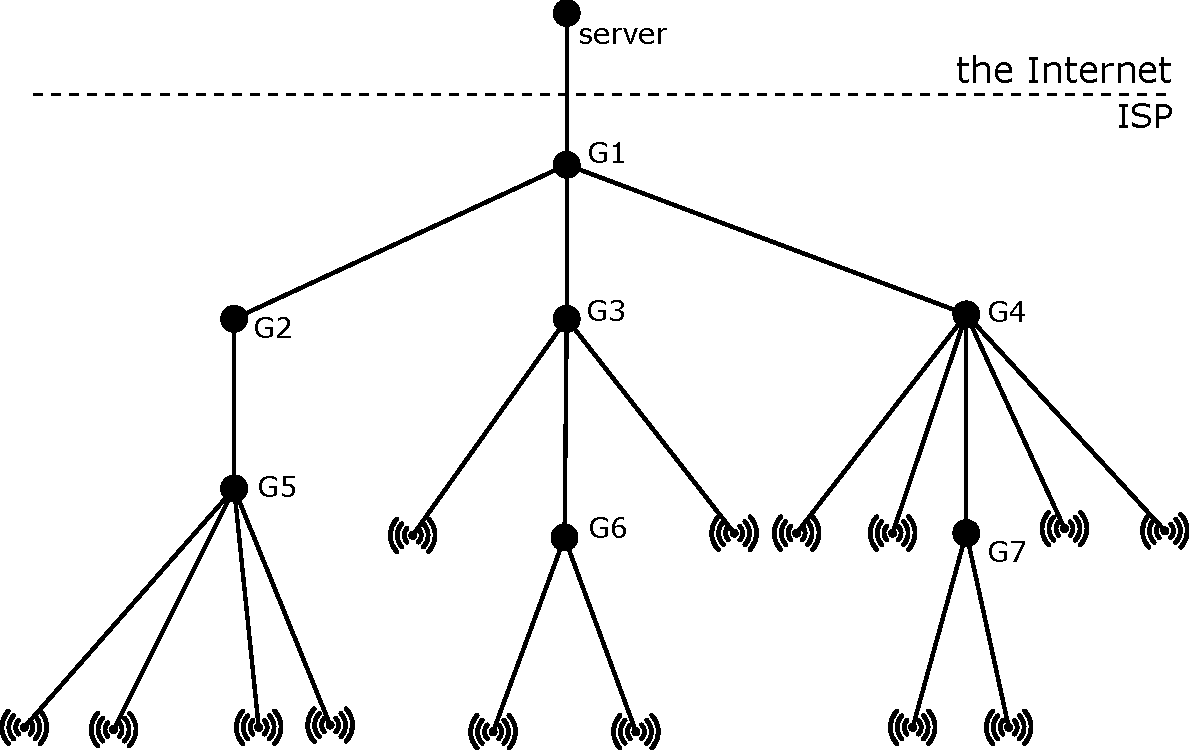
\includegraphics[width=137mm]{drawings/layout}
	\caption{The simulated network topology}
	\label{fig11:sim_layout}
\end{figure}


The simulated network is illustrated in Figure \ref{fig11:sim_layout}. The network is tree-shaped. The topmost node is server, it represents the rest of the Internet. Further, there is part of the infrastructure of an ISP. There are gateway nodes G1-G7. All gateways have 2-5 children. The leafs of this tree are access points (AP) of wireless networks. Finally, 8-12 clients (customers of ISP) are connected to each AP, with the default seed this results in 143 clients. 

Each client is connected to exactly one AP. The clients are connected with 802.11ac Wi-Fi --- they share the Wi-Fi bandwidth. APs and gateways are connected with point-to-point links with 100Mbps bandwidth and 5ms delay. The server is connected to G1 with 1000Mbps link with 50ms delay.

The clients download and upload data. All the traffic flows between the server and one of the clients. There are several types of applications that model various behaviour of real-life clients. The types are listed in table \ref{tab01:traffic}. They vary in transport protocol used, size of a single packet and the data rate at which they generate traffic. The data rate may be constant --- in that case the application generates packets on regular basis (e.g. it sends a packet every 5 milliseconds), or it may be variable.

The applications with variable bit rate turn on and off on irregular basis. During off period, it sends zero packets and during on time it sends packets at configured constant rate. The on times and off times are generated randomly --- using normal distribution $\mathcal{N}(1,1)$.

The count ratio column specifies the ratio of number of applications installed per type. The values in the \autoref{tab:traffic} mean, that there are 30 times more HTTP flows than SSH flows. We set the total number of applications to 280 --- roughly 2 applications are installed on every client. 

\begin{table}
	\caption{Types of flows used in the simulations}
	\label{tab:traffic}
	\centering
	
	\begin{tabular}{@{}lllllll@{}}
		\toprule
		Name     & Protocol & Data rate & C/VBR & directions & Packet  & Count \\
		         &          &           &       &            & size(B) & ratio \\ \midrule
		SSH      & TCP      & 1 kbps    & CBR   & both       & 20      & 1     \\
		VoIP     & TCP      & 60 kbps   & CBR   & both       & 208     & 1     \\
		Game     & TCP      & 100 kbps  & CBR   & both       & 512     & 1     \\
		TV       & TCP      & 3 Mbps    & CBR   & down only  & 1450    & 3     \\
		HTTP     & TCP      & unlimited & VBR   & down only  & 256     & 20    \\
		Download & TCP      & unlimited & CBR   & down only  & 1450    & 5     \\
		torrent  & UDP      & unlimited & CBR   & down only  & 1450    & 3     \\ \bottomrule
	\end{tabular}
\end{table}



To evaluate MSFC, we ran multiple simulations with different schedulers. Each time, we installed the evaluated scheduler to all nodes (NetDevices) of the simulation. We tested PfifoFast, CoDel, FQ CoDel and MSFC. We have used all schedulers with default parameters. 

We measured throughput, packet loss, delay and jitter using ns-3 module FlowMonitor \cite{flowMonitor}. Throughput is the rate at which packets flow through a node measured in bytes per second. Delay is the time taken to transmit a packet from sender to receiver. Jitter is variation of delay. FlowMonitor computes jitter of a packet simply, only relatively to the previous packet:
\[
	\text{\emph{Jitter}}(P_N) = \abs{\text{\emph{Delay}}(P_N) - \text{\emph{Delay}}(P_{N-1})},
\]
where $P_N$ is the n-th received packet. We measure all the values in the IP layer. That means we count in IP header, but not frame header (link layer header). Also, TCP--retransmitted packets count separately.

Using the testbed described, we ran several simulations with slightly different prioritization of flows. In each simulation, we assigned the same priority to all flows of the same type. We configured the simulation duration to 100 seconds.

Also, we only present results of 'download' direction --- the upload direction does not have enough throughput, and since we use full--duplex point-to-point links, the results are not interesting. The traffic schedulers do not have effect, if the network has enough bandwidth to transmit all potential traffic. 






\section{Simulation A}

\todo{rozlozenie obrazkov a tabuliek na stranky a ich poradie}
 
%\begin{table}
	\caption{Prioritization of flows in simulations.}
	\label{tab:flows_prio}
	\centering
	
	\begin{tabular}{@{}lc@{}}
		\toprule
        Application     & Priority in     \\ 
        type            & simulation A    \\ \midrule
        SSH             & 2               \\
        VoIP            & 2               \\
        Game            & 2               \\
        TV              & 2               \\
        HTTP            & 1               \\
        Download        & 0               \\
        Torrent         & 0               \\ \bottomrule
	\end{tabular}
\end{table}

\begin{table}
	\caption{Priorities assigned to types of flows and resulting number of flows in simulation A.}
	\label{tab:flows_count_A}
	\centering
	
	\begin{tabular}{@{}l|cccc@{}}
		\toprule
		\multicolumn{1}{c|}{Application} & Priority & \multicolumn{3}{c}{Number of flows}  \\
		\multicolumn{1}{c|}{type}        &          & Priority 0 & Priority 1 & Priority 2 \\ \midrule
		SSH                              &    2     &     0      &     0      &     9      \\
		VoIP                             &    2     &     0      &     0      &     9      \\
		Game                             &    2     &     0      &     0      &     9      \\
		TV                               &    2     &     0      &     0      &     27     \\
		HTTP                             &    1     &     0      &    162     &     0      \\
		Download                         &    0     &     40     &     0      &     0      \\
		Torrent                          &    0     &     24     &     0      &     0      \\ \midrule
		Total                            &          &     64     &    162     &     54     \\ \bottomrule
	\end{tabular}
\end{table}

\begin{table}[]
	\centering
	\begin{tabular}{@{}lllll@{}}
		\toprule
								& CoDel & FQ CoDel & MSFC & pfifo\_fast  \\ \midrule
		Throughput (kbps)       & 290066    & 290264 & 290228   & 290613 \\
		Delay (ms)              & 94.4      & 75.2   & 75.0     & 163.1    \\
		Jitter (ms)             & 0         & 2      & 2        & 0      \\
		Packet Loss (packets)   & 86731     & 1571844& 1719122  & 68259  \\ \bottomrule
	\end{tabular}
	\caption{Overall results of the simulation. The table shows average network throughput in kilobits per second, harmonic mean of packet delay in milliseconds, arithmetic mean of packet jitter in milliseconds and the total number of packets lost.}
	\label{tab:results_A}
\end{table}


\begin{table}
	\centering
	
	\begin{tabular}{@{}l|rrrr@{}}
		\toprule
						& CoDel & FQ CoDel & MSFC & pfifo\_fast  \\ \midrule
		SSH             &     257       &     64        &     64        &     183       \\
		VoIP            &     108       &     66        &     67        &     160       \\
		Game            &     139       &     65        &     65        &     163       \\
		TV              &     124       &     69        &     66        &     155       \\
		HTTP            &     108       &     73        &     76        &     153       \\
		Download        &     105       &     69        &     77        &     150       \\
		Torrent         &     207       &     2448      &     1249      &     178       \\ \bottomrule
	\end{tabular}
	\caption{Average delay of individual types of flows in milliseconds.}
	\label{tab:delay_A}
\end{table}

\begin{table}
	\centering
	
	\begin{tabular}{@{}l|rrrrr@{}}
		\toprule
		         & {CoDel} & {FQ CoDel} &  {MSFC} & {pfifo\_fast} &  \\ \midrule
		SSH      &      48 &          0 &       0 &          1709 &  \\
		VoIP     &     167 &          0 &       0 &           311 &  \\
		Game     &     197 &          3 &       0 &           488 &  \\
		TV       &     979 &        719 &       2 &          3124 &  \\
		HTTP     &    5239 &       3670 &    5107 &         14232 &  \\
		Download &    1360 &       1099 &    1169 &          4923 &  \\
		Torrent  &   78741 &    1566353 & 1712844 &         43472 &  \\ \bottomrule
	\end{tabular}
	\caption{Number of lost packets by flow types.}
	\label{tab:loss_A}
\end{table}

\begin{table}
	\centering
	
	\begin{tabular}{@{}l|rrrrr@{}}
		\toprule
		         & {Data rate} & {CoDel} & {FQ CoDel} &  {MSFC} & {pfifo\_fast} \\ \midrule
		SSH      &           1 &    3.60 &       3.51 &    3.51 &          3.41 \\
		VoIP     &          60 &   66.47 &      73.04 &   73.04 &         57.47 \\
		Game     &         100 &   80.67 &     107.43 &  107.44 &         66.71 \\
		TV       &        3000 &  270.50 &    1327.67 & 3185.29 &        265.41 \\
		HTTP     &   unlimited &  231.41 &     919.32 &  790.60 &        220.30 \\
		Download &   unlimited &  362.88 &    1311.46 &  908.10 &        328.85 \\
		Torrent  &   unlimited & 9558.39 &    2140.52 & 1590.36 &       9727.35 \\ \bottomrule
	\end{tabular}
	\caption{Average throughput of individual flows sorted by flow types in kilobits per second (kbps).}
	\label{tab:throughput_A}
\end{table}












In simulation A, we assigned priorities to types of flows according to in Table \ref{tab:flows_count_A}. The Table \ref{tab:flows_count_A} shows also number of flows of individual types. It is the result of the flow priorities, the count ratio from Table \ref{tab:traffic} and maximum number of flows equal to 280.  


The overall results of simulation A are shown in Table \ref{tab:results_A}. It gives us general overview, however the average of delay and packet loss does not represent the data well. Table \ref{tab:delay_A} shows average delay of types of flows, Table \ref{tab:loss_A} shows number of lost packets and Table \ref{tab:throughput_A} shows how much throughput receive an average flow of particular type.

We will shed some light on all the numbers. The throughput of the torrent flows in one--queue schedulers CoDel and pfifo\_fast is dramatically higher than FQ CoDel and MSFC. That naturally results in all other flows receiving less throughput, since all schedulers manage to utilize the links similarly (throughput row in Table \ref{tab:results_A}). The reason is, that UDP does not have any congestion control and thus sends as much packets as possible regardless of being dropped. CoDel and pfifo\_fast mix all the packets in one queue so the TCP flows notice the congestion and slow down. The result is, that misbehaving users are actually favored. FQ CoDel and MSFC employ fair queueing (see \autoref{sec:fair_queueing}) principles that isolate the misbehaving users.

The Tables \ref{tab:delay_A} and \ref{tab:loss_A} with delay and loss statistics confirm the same. CoDel and pfifo\_fast have higher delay of all flows, while FQ CoDel and MSFC manage to keep low delay of all TCP flows and isolate the UDP flows. 

Additionally, because the average of packet delay may be too generalising, we present its distribution in Figure \ref{fig:overall_delay} Here we can see, that arithmetic mean does not represent the delay well, because there are few packets (less than 7\%) of the torrent type in FQ CoDel, CoDel and MSFC that have delay over 3 seconds. The Figure \ref{fig:torrent_delay} shows the distribution of torrent packets to illustrate the extreme delay.

The measured jitter is close to zero. The average values of 0-2 from Table \ref{tab:results_A} represent the jitter well and jitter of all types of flows was negligible --- always less than 6\% of delay.

Another thing we can observe is, that MSFC responds to the assigned priorities well. SSH, VoIP and Game flows achieved almost the same quality of service. Not surprisingly, since we assigned the highest priority to TV flows, average TV flow received 3185 kbps with MSFC, which is much more than 1327 kbps it got from FQ CoDel. Of course, the rest of flows with lesser priorities had less throughput, but the decrease again scaled with the priorities.

Figure \ref{fig:delay_flows} shows detailed comparison of delays of FQ CoDel and MSFC (we do not compare CoDel and pfifo\_fast, since their delay was much higher).


\begin{figure}
	\centering
	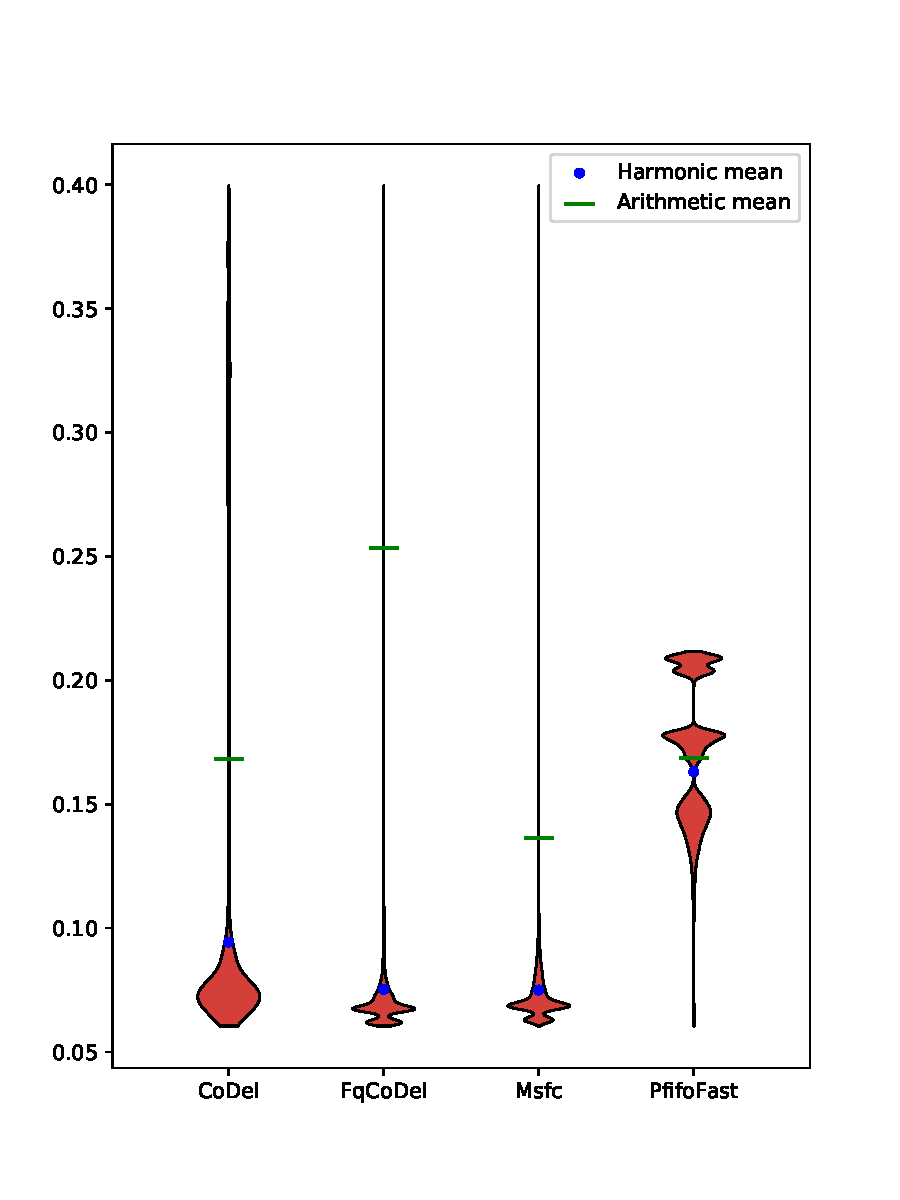
\includegraphics[width=137mm]{drawings/overall-delay-down}
	\caption{The distribution of delay in seconds. Packets with delay higher than 0.4 seconds are omitted in the distribution, but the means are computed from all values. This restriction results in displaying 93\% of data. However, the few packets have such high delay, that it considerably affects the arithmetic means. }
	
	\label{fig:overall_delay}
\end{figure}

\begin{figure}
	\centering
	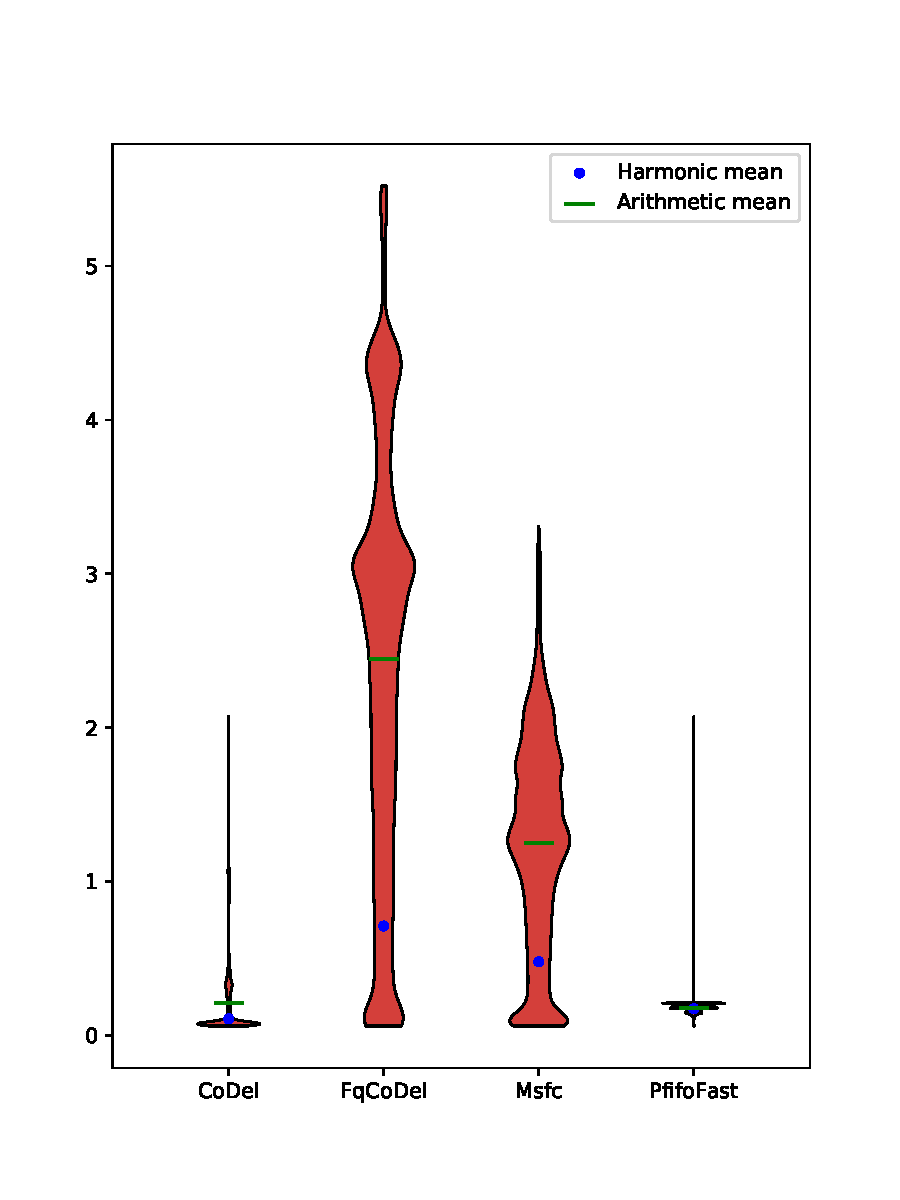
\includegraphics[width=137mm]{drawings/type6-delay-down}
	\caption{The distribution of delay of torrent packets in seconds.}
	\label{fig:torrent_delay}
\end{figure}



\begin{figure*}
	\centering
	\begin{subfigure}[b]{0.475\textwidth}
		\centering
		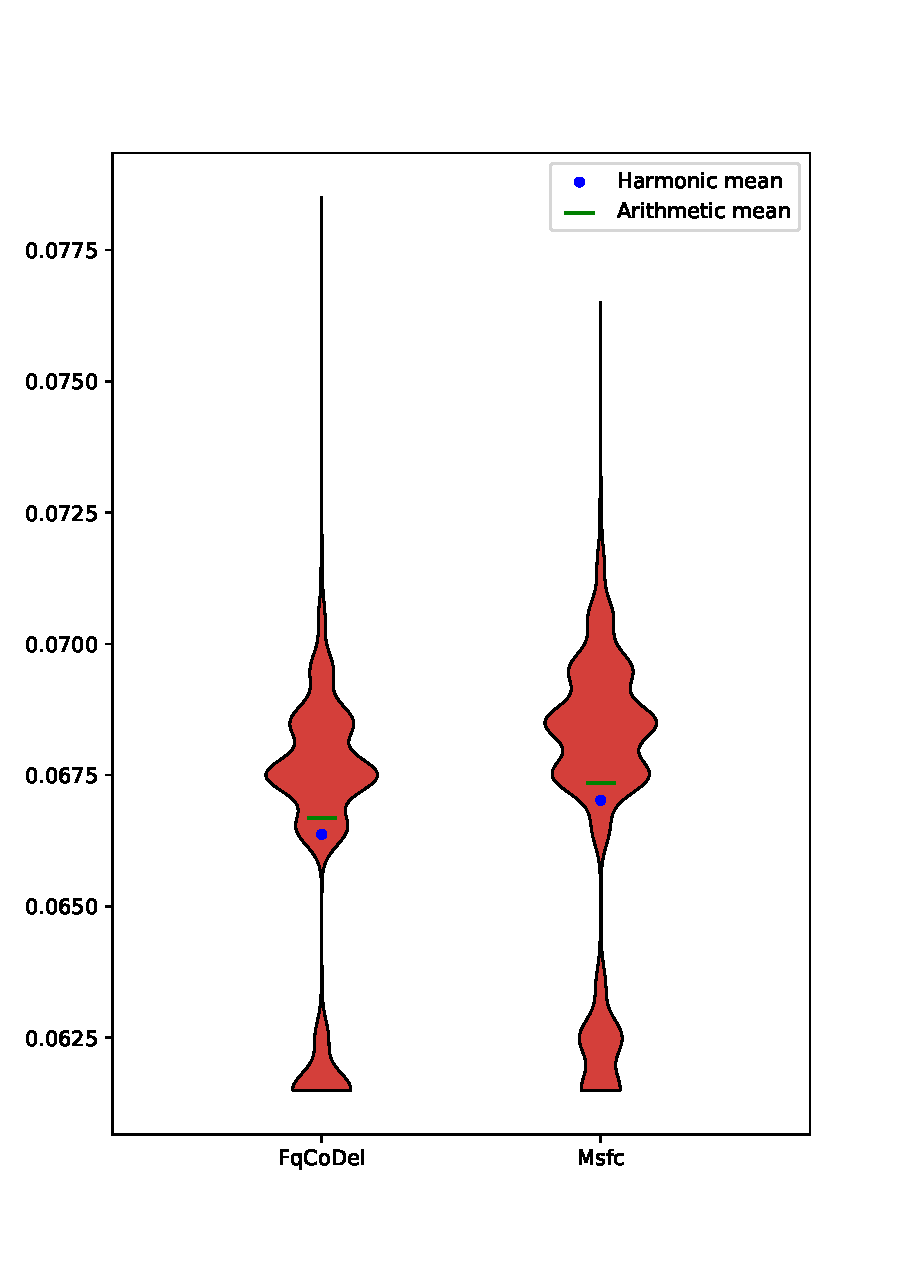
\includegraphics[width=\textwidth]{drawings/type1-delay-down}
		\caption[]%
		{{\small Delay of VoIP flows}}    
		\label{fig:delay_voip}
	\end{subfigure}
	\hfill
	\begin{subfigure}[b]{0.475\textwidth}  
		\centering 
		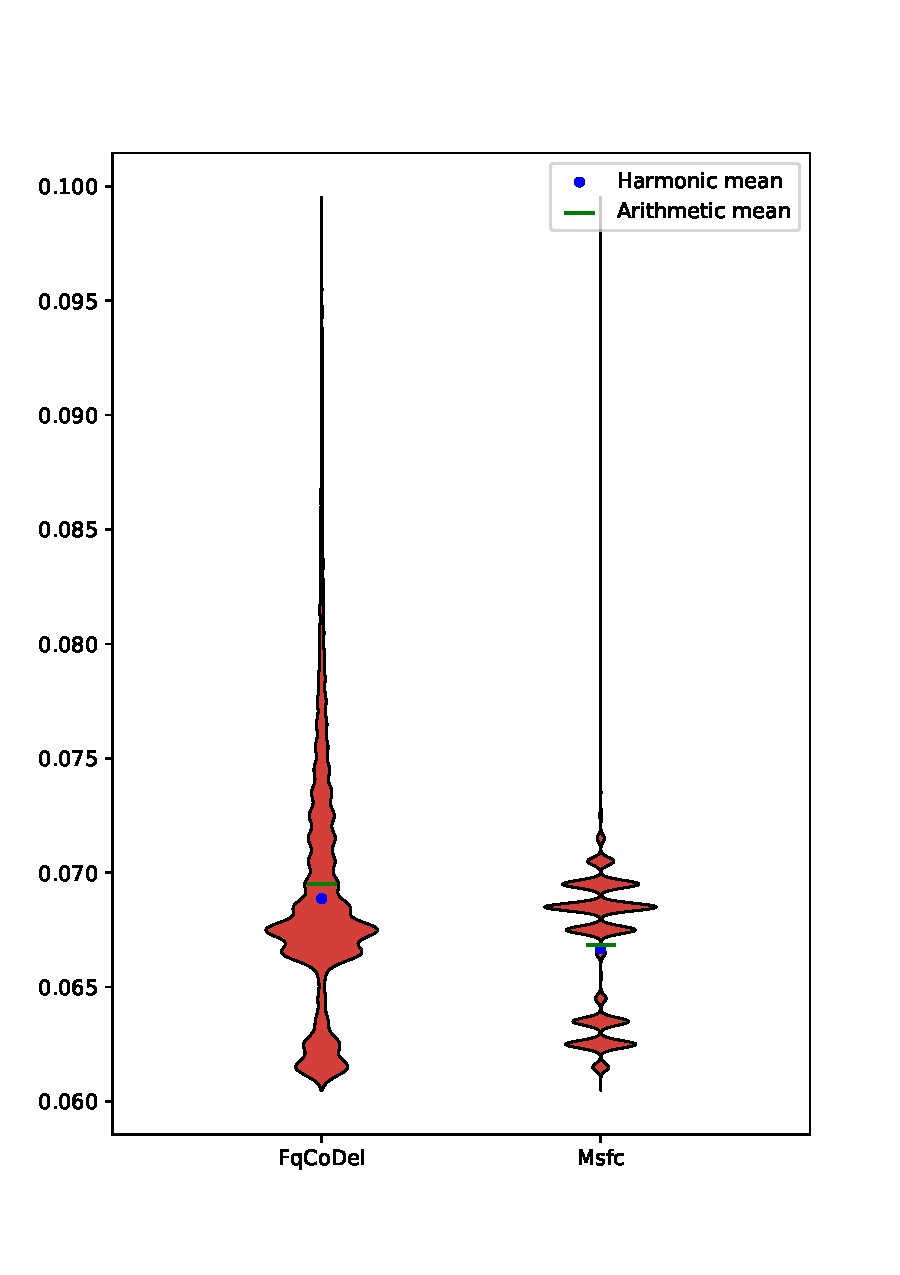
\includegraphics[width=\textwidth]{drawings/type3-delay-down}
		\caption[]%
		{{\small Delay of TV flows}}    
		\label{fig:delay_tv}
	\end{subfigure}
	\par\bigskip % force a bit of vertical whitespace
	\begin{subfigure}[b]{0.475\textwidth}   
		\centering 
		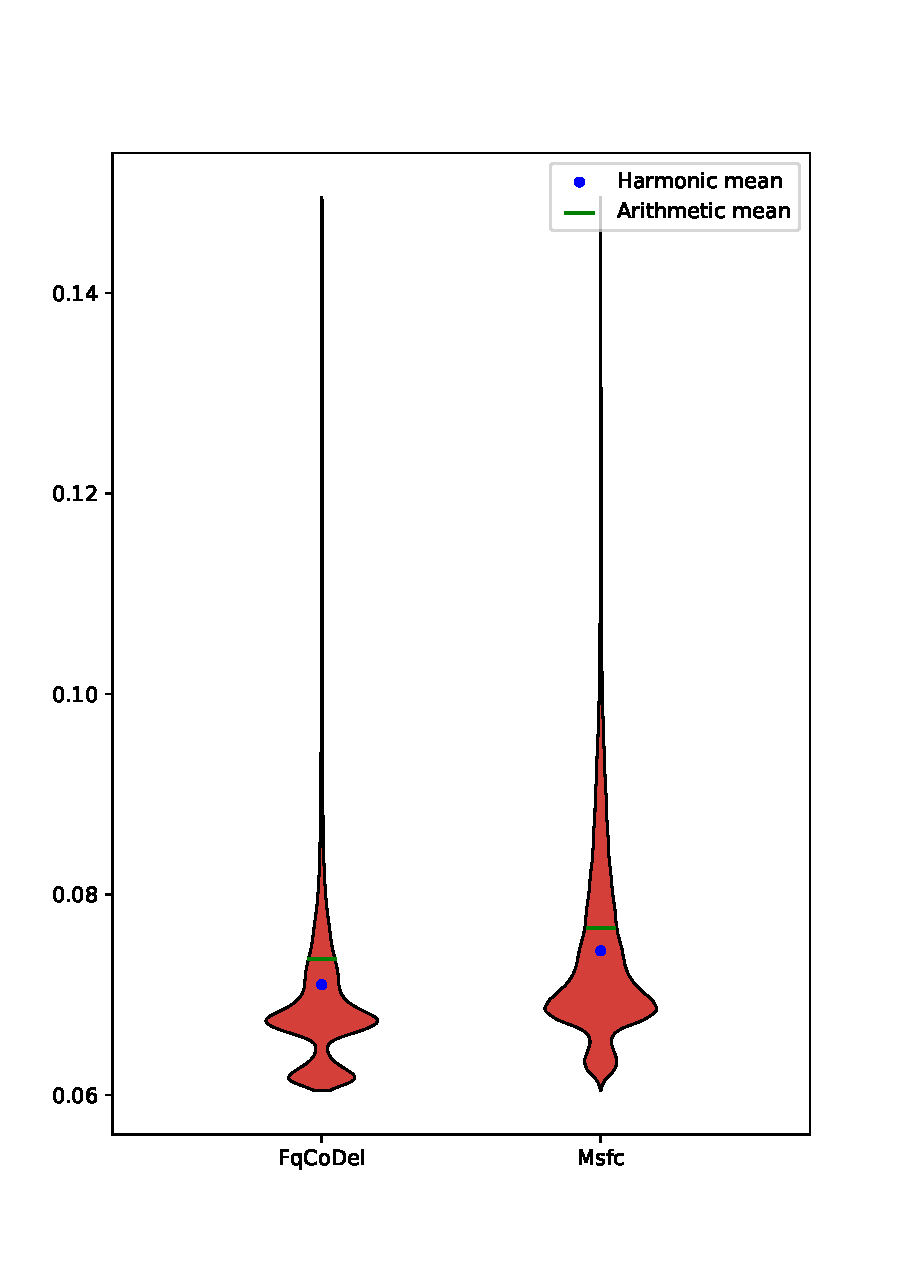
\includegraphics[width=\textwidth]{drawings/type4-delay-down}
		\caption[]%
		{{\small Delay of HTTP flows}}    
		\label{fig:delay_http}
	\end{subfigure}
	\quad
	\begin{subfigure}[b]{0.475\textwidth}   
		\centering 
		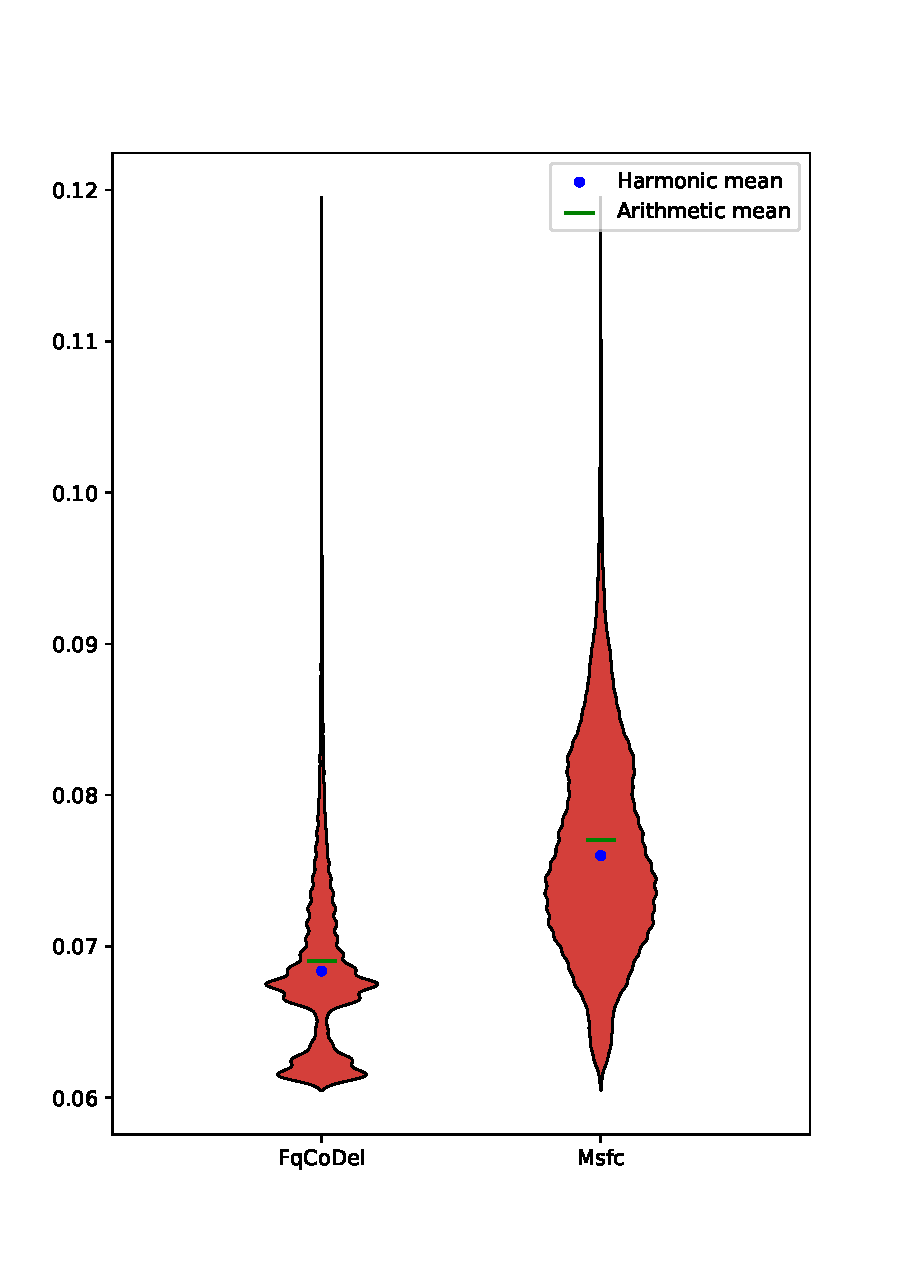
\includegraphics[width=\textwidth]{drawings/type5-delay-down}
		\caption[]%
		{{\small Delay of Download flows}}    
		\label{fig:delay_download}
	\end{subfigure}
	\caption[]
	{\small The distribution of delay of different types of flows. We omit few extreme values to get better visualization, however the means are calculated from all values.} 
	\label{fig:delay_flows}
\end{figure*}





\clearpage
\subsection{Simulation B}

\begin{table}
	\caption{Priorities assigned to types of flows and resulting number of flows in simulation B.}
	\label{tab:flows_count_B}
	\centering
	
	\begin{tabular}{@{}l|cccc@{}}
		\toprule
		\multicolumn{1}{c|}{Application} & Priority & \multicolumn{3}{c}{Number of flows}   \\
		\multicolumn{1}{c|}{type}        &          & Priority 0 & Priority 1 & Priority 2  \\ \midrule
		SSH                              &    2     &     0      &     0      &     9       \\
		VoIP                             &    2     &     0      &     0      &     9       \\
		Game                             &    2     &     0      &     0      &     9       \\
		TV                               &    1     &     0      &     27     &     0       \\
		HTTP                             &    1     &     0      &    162     &     0       \\
		Download                         &    1     &     0      &     40     &     0       \\
		Torrent                          &    0     &     24     &     0      &     0       \\ \midrule
		Total                            &          &     24     &    229     &     27      \\ \bottomrule
	\end{tabular}
\end{table}


In second simulation we demonstrate that assigning the priorities to flows may not be as straightforward as it may seem when using MSFC. We ran the simulation with priorities according to Table \ref{tab:flows_count_B}. The overall results of the simulation is shown in Table \ref{tab:results_B}. The performance of all schedulers except MSFC remained unchanged, since MSFC is the only scheduler that takes priorities into consideration.

The comparisons of delay, loss and throughput are shown in Tables \ref{tab:delay_B}, \ref{tab:loss_B} and \ref{tab:throughput_B}. The biggest difference is noticeable in the throughput of torrent flows. With this priority assignment, MSFC gave torrent almost two times higher throughput than FQ CoDel, although we assigned the lowest priority to the torrent flows. All the priority 1 flows have less throughput and worse delay. This unpleasant behaviour is caused by the distribution of flows into the priorities (see Table \ref{tab:flows_count_B}) and the fact, that MSFC treats flows of different priority classes absolutely separately. There are too many flows, that 'fight' for the bandwidth of priority 1 class, while there are few flows, that have whole priority 0 class reserved for them.

The priority 2 flows results ended up without any notable difference. Also it is worth mentioning, that even though we assigned flows with low data rate to the priority 2 class, which reserves huge bandwidth, it did not affect the overall throughput negatively. When packets of the highest priority class were not available, its bandwidth was assigned to the rest of priority classes.


\begin{table}[]
	\centering
	\begin{tabular}{@{}lrrrr@{}}
		\toprule
								& CoDel & FQ CoDel & MSFC & pfifo\_fast  \\ \midrule
		Throughput (kbps)       & 290066    & 290264 & 290372   & 290613 \\
		Delay (ms)              & 94.4      & 75.2   & 85.9     & 163.1    \\
		Jitter (ms)             & 0         & 2      & 2        & 0      \\
		Packet Loss (packets)   & 86731     & 1571844& 1180488  & 68259  \\ \bottomrule
	\end{tabular}
	\caption{Overall results of simulation B. The table shows average network throughput in kilobits per second, harmonic mean of packet delay in milliseconds, arithmetic mean of packet jitter in milliseconds and the total number of packets lost.}
	\label{tab:results_B}
\end{table}


\begin{table}

	\centering
	
	\begin{tabular}{@{}l|rrrr@{}}
		\toprule
						& CoDel & FQ CoDel & MSFC & pfifo\_fast  \\ \midrule
		SSH             &     257       &     64        &     64        &     183       \\
		VoIP            &     108       &     66        &     66        &     160       \\
		Game            &     139       &     65        &     64        &     163       \\
		TV              &     124       &     69        &     73        &     155       \\
		HTTP            &     108       &     73        &     75        &     153       \\
		Download        &     105       &     69        &     77        &     150       \\
		Torrent         &     207       &     2448      &     936      &     178       \\ \bottomrule
	\end{tabular}
	\caption{Average delay of individual types of flows in milliseconds in simulation B.}
	\label{tab:delay_B}
\end{table}

\begin{table}
	\centering
	
	\begin{tabular}{@{}l|rrrrr@{}}
		\toprule
		& {CoDel} & {FQ CoDel} & {MSFC} & {pfifo\_fast}  \\ \midrule
		SSH       &    48         &    0          &    0          &    1709  \\
		VoIP      &    167        &    0          &    0          &    311   \\
		Game      &    197        &    3          &    0          &    488   \\
		TV        &    979        &    719        &    1009       &    3124  \\
		HTTP      &    5239       &    3670       &    4187       &    14232 \\
		Download  &    1360       &    1099       &    1440       &    4923  \\
		Torrent   &    78741      &    1566353    &    1173852    &    43472 \\ \bottomrule
	\end{tabular}
	\caption{Number of lost packets by flow types in simulation B.}
	\label{tab:loss_B}
\end{table}

\begin{table}
	\centering
	\begin{tabular}{@{}l|rrrrr@{}}
		\toprule
		         & {Data rate} & {CoDel} & {FQ CoDel} &  {MSFC} & {pfifo\_fast} \\ \midrule
		SSH      &           1 &    3.60 &       3.51 &    3.51 &          3.41 \\
		VoIP     &          60 &   66.47 &      73.04 &   73.02 &         57.47 \\
		Game     &         100 &   80.67 &     107.43 &  107.44 &         66.71 \\
		TV       &        3000 &  270.50 &    1327.67 &  967.26 &        265.41 \\
		HTTP     &   unlimited &  231.41 &     919.32 &  758.23 &        220.30 \\
		Download &   unlimited &  362.88 &    1311.46 &  962.31 &        328.85 \\
		Torrent  &   unlimited & 9558.39 &    2140.52 & 4219.79 &       9727.35 \\ \bottomrule
	\end{tabular}
	\caption{Average throughput of individual flows sorted by flow types in kilobits per second (kbps) in simulation B.}
	\label{tab:throughput_B}
\end{table}












\begin{figure*}
	\centering
	\begin{subfigure}[b]{0.475\textwidth}
		\centering
		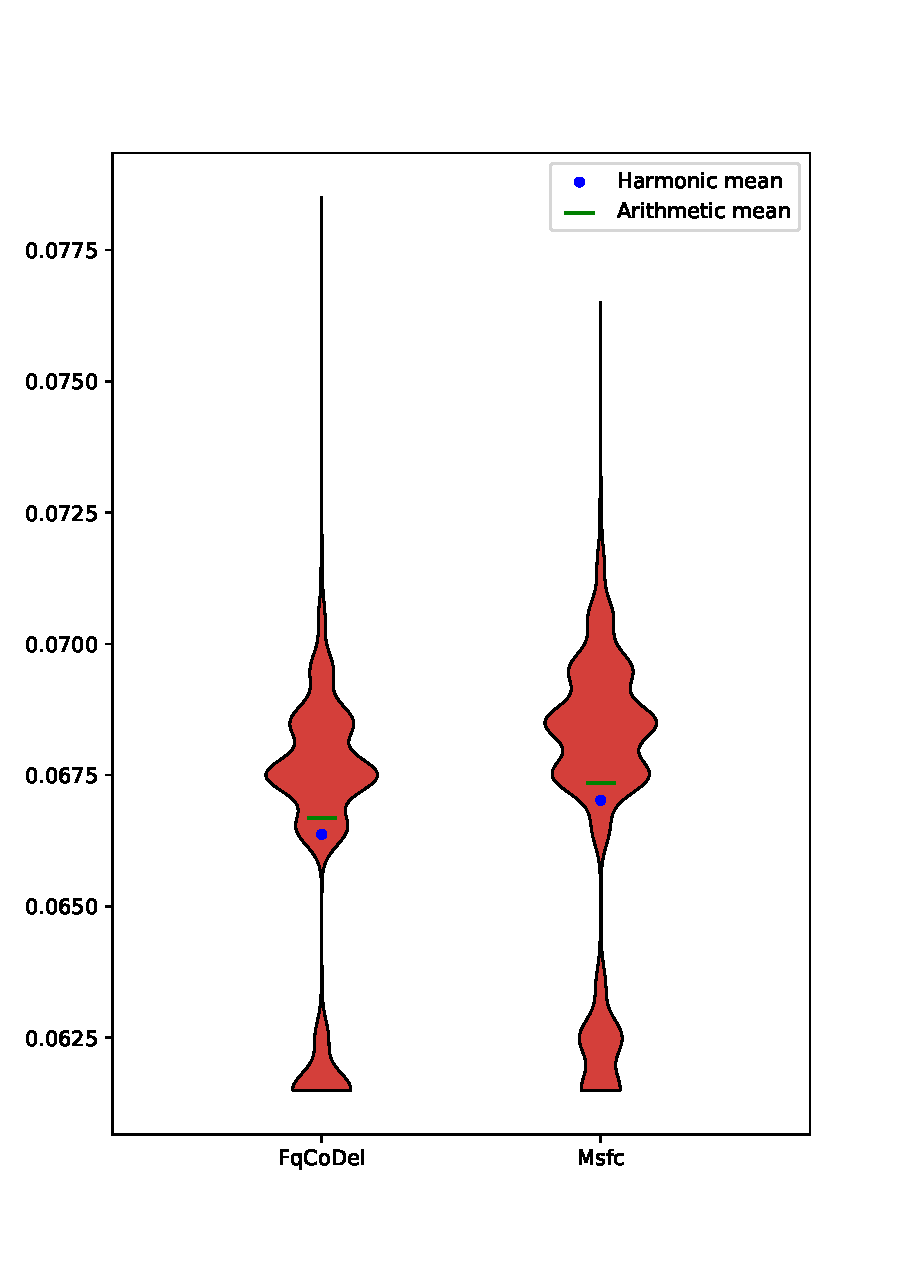
\includegraphics[width=\textwidth]{drawings/type1-delay-down}
		\caption[]%
		{{\small Delay of VoIP flows}}    
		\label{fig:delay_voip}
	\end{subfigure}
	\hfill
	\begin{subfigure}[b]{0.475\textwidth}  
		\centering 
		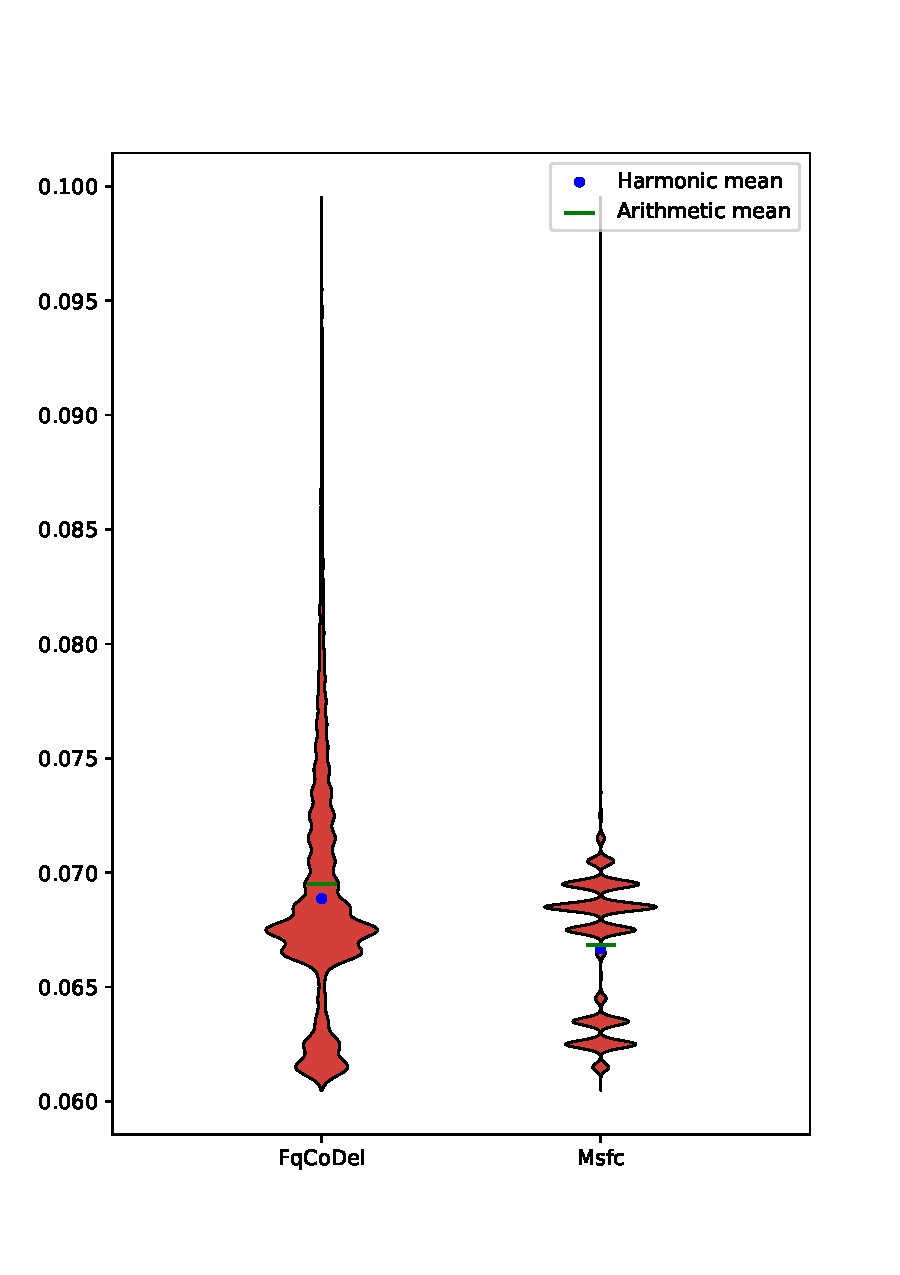
\includegraphics[width=\textwidth]{drawings/type3-delay-down}
		\caption[]%
		{{\small Delay of TV flows}}    
		\label{fig:delay_tv}
	\end{subfigure}
	\par\bigskip % force a bit of vertical whitespace
	\begin{subfigure}[b]{0.475\textwidth}   
		\centering 
		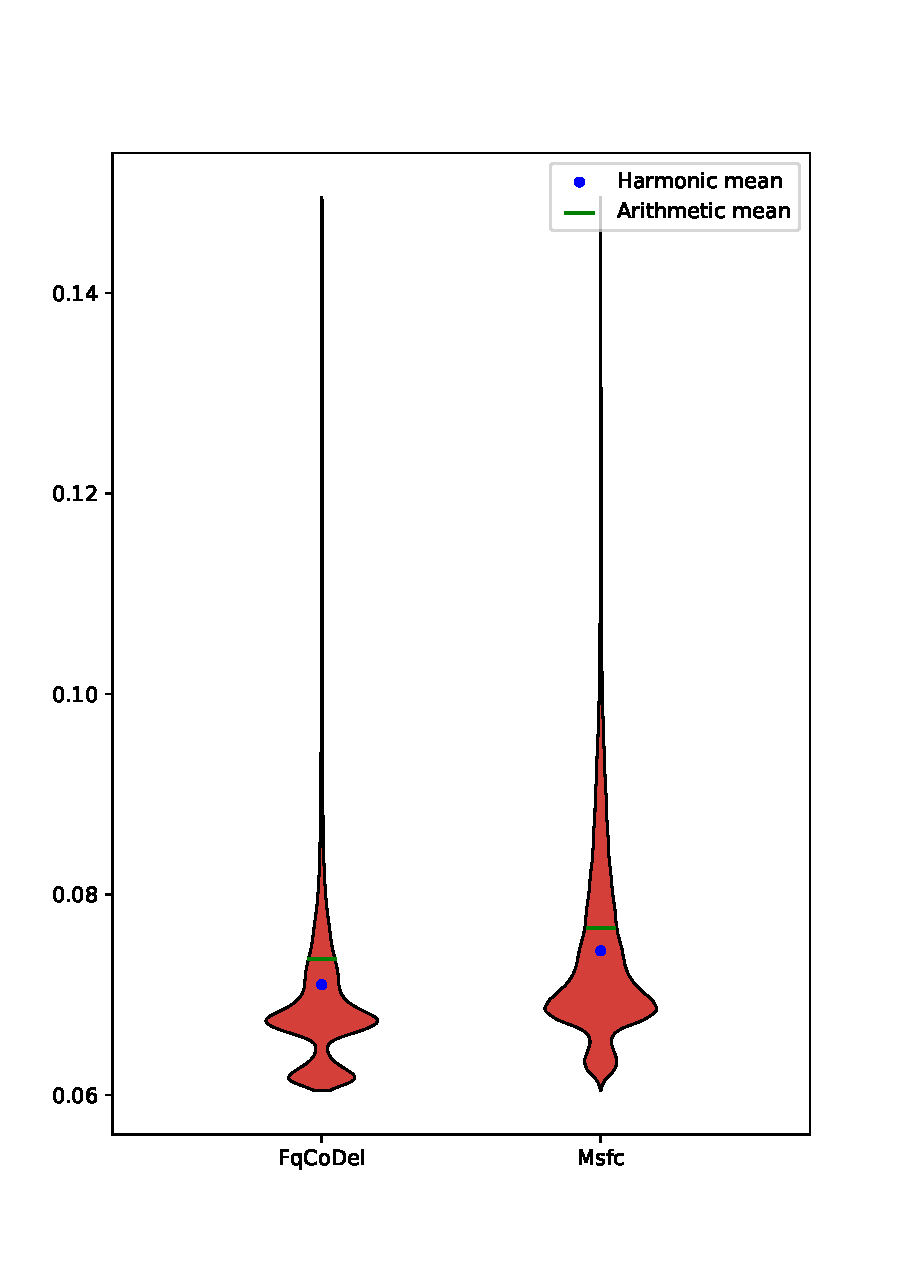
\includegraphics[width=\textwidth]{drawings/type4-delay-down}
		\caption[]%
		{{\small Delay of HTTP flows}}    
		\label{fig:delay_http}
	\end{subfigure}
	\quad
	\begin{subfigure}[b]{0.475\textwidth}   
		\centering 
		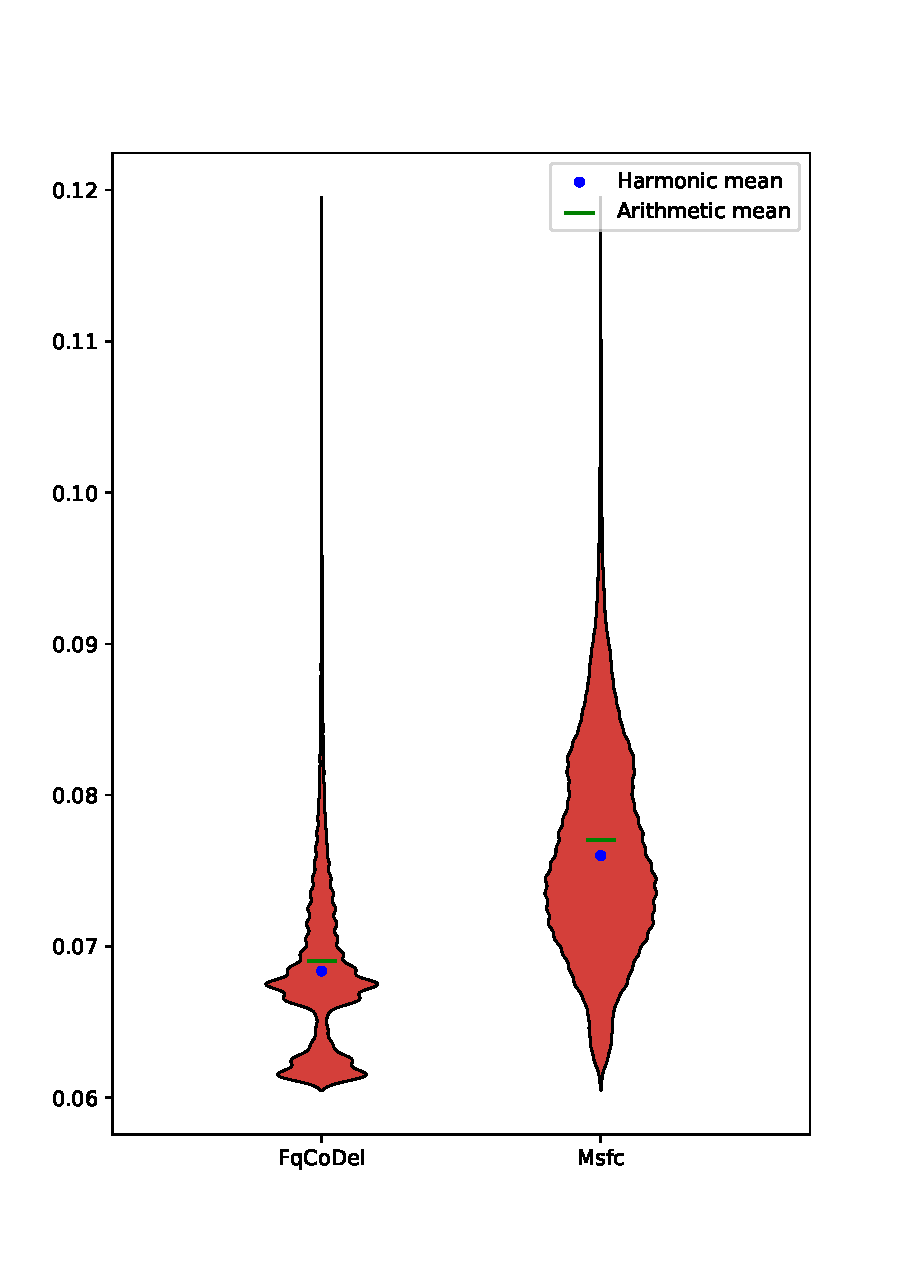
\includegraphics[width=\textwidth]{drawings/type5-delay-down}
		\caption[]%
		{{\small Delay of Download flows}}    
		\label{fig:delay_download}
	\end{subfigure}
	\caption[]
	{\small The distribution of delay of different types of flows. We omit few extreme values to get better visualization, however the means are calculated from all values.} 
	\label{fig:delay_flows}
\end{figure*}



\section{Discussion}










\chapter*{Conclusion}
\addcontentsline{toc}{chapter}{Conclusion}

In this thesis, we have described, implemented and benchmarked the Multilevel Stochastic Fairness CoDel --- a traffic scheduler built on the principles of fair queuing and CoDel, that is able to recognize categories of flows of various priorities. At the same time, the configuration is kept as simple as possible. 

In the \autoref{chap1} we have discussed issues connected to network scheduling and related research. We have described basic qualities that can be measured in packet-switching networks commonly referred to as QoS. We described the bufferbloat and schedulers that aimed to mitigate its consequences: RED and CoDel. Next, we described the the need of fairness in networks as well as means to achieve it. Finally, we have taken a look at a traffic scheduler from a different category: HTB is a classful scheduler that uses hierarchical configuration to differentiate between categories of flows present in the network.

In the \autoref{chap02} we have described the MSFC as well as its implementations: for Linux operating system and for ns-3. Firstly, we have provided a brief overview of the Linux kernel API that every traffic scheduler must implement in order to describe the existing Linux implementation of MSFC written by supervisor of this thesis. Secondly, we have taken a look at the model of Network Simulator 3, its API for traffic scheduling and finally the MSFC implementation.

In the \autoref{chap3} we have designed a simulation in order to benchmark MSFC. We have compared it to CoDel, FQ CoDel and pfifo\_fast. We have simulated a tree-shaped network similar to wireless-based ISP infrastructure and installed the benchmarked scheduler to all nodes of the network. We generated the same traffic in each run and measured the impact of traffic scheduler choice on quality of service.

The simulation results showed that MSFC can be easily used to prioritize important traffic and services that have high requirements on network resources. To achieve this we did not use any information about the traffic shape; We only assigned higher priority to some of the flows.



\section*{Future work}
\addcontentsline{toc}{section}{Future work}





%%% Bibliography
%%% Bibliography (literature used as a source)
%%%
%%% We employ bibTeX to construct the bibliography. It processes
%%% citations in the text (e.g., the \cite{...} macro) and looks up
%%% relevant entries in the bibliography.bib file.
%%%
%%% The \bibliographystyle command selects, which style will be used
%%% for references from the text. The argument in curly brackets is
%%% the name of the corresponding style file (*.bst). Both styles
%%% mentioned in this template are included in LaTeX distributions.

% \bibliographystyle{plainnat}    %% Author (year)
% \bibliographystyle{unsrt}     %% [number]
\bibliographystyle{alpha}

\renewcommand{\bibname}{Bibliography}

%%% Generate the bibliography. Beware that if you cited no works,
%%% the empty list will be omitted completely.

\bibliography{bibliography}

%%% If case you prefer to write the bibliography manually (without bibTeX),
%%% you can use the following. Please follow the ISO 690 standard and
%%% citation conventions of your field of research.

% \begin{thebibliography}{99}
%
% \bibitem{lamport94}
%   {\sc Lamport,} Leslie.
%   \emph{\LaTeX: A Document Preparation System}.
%   2nd edition.
%   Massachusetts: Addison Wesley, 1994.
%   ISBN 0-201-52983-1.
%
% \end{thebibliography}



%%% Figures used in the thesis (consider if this is needed)
\listoffigures

%%% Tables used in the thesis (consider if this is needed)
%%% In mathematical theses, it could be better to move the list of tables to the beginning of the thesis.
\listoftables

%%% Abbreviations used in the thesis, if any, including their explanation
%%% In mathematical theses, it could be better to move the list of abbreviations to the beginning of the thesis.
%\chapwithtoc{List of Abbreviations}
\renewcommand{\nomname}{List of Abbreviations}
%\printnomenclature

%%% Attachments to the bachelor thesis, if any. Each attachment must be
%%% referred to at least once from the text of the thesis. Attachments
%%% are numbered.
%%%
%%% The printed version should preferably contain attachments, which can be
%%% read (additional tables and charts, supplementary text, examples of
%%% program output, etc.). The electronic version is more suited for attachments
%%% which will likely be used in an electronic form rather than read (program
%%% source code, data files, interactive charts, etc.). Electronic attachments
%%% should be uploaded to SIS and optionally also included in the thesis on a~CD/DVD.
\chapwithtoc{Attachments}

\section*{Attachment A - the Enclosed CD}

On the CD attached to this thesis (and on the online Thesis Repository of Charles University \cite{TRepo}) we enclose
the source codes of the implemented software together with the source codes of its
dependencies (GNU Nettle and GMP), and also the code of the SIDH Library, so it can
be used for comparison when benchmarking.

The electronic version of this thesis is also enclosed.

\openright
\end{document}
